

What do I want to show in results section?

- cutflow

\begin{table}[h!]
\begin{center}
\renewcommand{\arraystretch}{1.2}
\resizebox{1.0\textwidth}{!}{
%\begin{tabular}{ +l^| c^ c^ c^ | c^ c^ c^ c^ c^ c }
\begin{tabular}{l || c c c | c c c c c c }
\hline
% & & & Total & & & & Non-$WW$ & & \\
\multirow{2}{*}{Cut stage} & \multirow{2}{*}{Observed} &
\multirow{2}{*}{Signal} & Total &
\multirow{2}{*}{top} & \multirow{2}{*}{$WW$} & \multirow{2}{*}{ggF} &
Non-$WW$ & \multirow{2}{*}{\ZDY} & \multirow{2}{*}{Fakes} \\
 & & & Back & & & & Diboson & & \\
\hline
$\Njet \geq 2$ & $676470 \pm 822$ & $134 \pm 2$ & $669892 \pm 1279$ &
$106081$ & $2779$ & $198$ & $1553$ & $556559$ & $2722$ \\
\hline
$\emme~\textrm{channel}$ & $61434 \pm 248$ & $64 \pm 1$ & $59597 \pm
39$ & $53196$ & $1423$ & $103$ & $378$ & $3356$ & $1142$ \\
\ $\Nbjet = 0$ & $7818 \pm 88$ & $47 \pm 1$ & $7569 \pm 23$ & $3232$ &
$1036$ & $76$ & $272$ & $2460$ & $493$ \\
\ $\textrm{CJV}$ & $6313 \pm 79$ & $40 \pm 1$ & $6097 \pm 21$ & $2462$ &
$859$ & $61$ & $226$ & $2083$ & $408$ \\
\ $\textrm{OLV}$ & $1264.0 \pm 35.6$ & $22.7 \pm 0.4$ & $1273.5 \pm 8.7$
& $542.8$ & $156.1$ & $17.8$ & $45.7$ & $434.5$ & $76.5$ \\
\ $Z\rightarrow{\tau\tau}~\textrm{veto}$ & $718.0 \pm 26.8$ & $16.8 \pm
0.3$ & $703.0 \pm 5.7$ & $369.6$ & $101.1$ & $13.8$ & $31.2$ & $134.5$
& $52.8$ \\
\hline
\ $\textrm{BDT} > -0.48$ & $57.0 \pm 7.5$ & $11.7 \pm 0.2$ & $44.2 \pm
1.3$ & $16.4$ & $8.6$ & $4.6$ & $3.5$ & $5.3$ & $5.8$ \\
\hline
$\eemm~\textrm{channel}$ & $615036 \pm 784$ & $70 \pm 1$ & $607896 \pm
1278$ & $50497$ & $1356$ & $95$ & $1175$ & $553203$ & $1569$ \\
\ $\calomet > 45 \gev$ & $119456 \pm 346$ & $45 \pm 1$ & $118395 \pm
443$ & $38710$ & $1025$ & $60$ & $736$ & $77376$ & $488$ \\
\ $\trkmet > 40 \gev$ & $58672 \pm 242$ & $39 \pm 1$ & $56435 \pm 207$
& $35832$ & $944$ & $51$ & $640$ & $18560$ & $408$ \\
\ $Z \textrm{veto}$ & $34339 \pm 185$ & $35 \pm 1$ & $33174 \pm 59$ &
$28358$ & $756$ & $50$ & $177$ & $3509$ & $323$ \\
\ $\mll < 75 \gev$ & $19552 \pm 140$ & $32 \pm 1$ & $18330 \pm 39$ &
$14811$ & $365$ & $50$ & $105$ & $2743$ & $256$ \\
\ $\Nbjet = 0$ & $3367 \pm 58$ & $24 \pm 0$ & $3214 \pm 30$ & $879$ &
$265$ & $36$ & $72$ & $1900$ & $62$ \\
\ $\textrm{CJV}$ & $2653 \pm 52$ & $20 \pm 0$ & $2515 \pm 28$ & $671$ &
$219$ & $29$ & $59$ & $1489$ & $49$ \\
\ $\textrm{OLV}$ & $664.0 \pm 25.8$ & $12.2 \pm 0.2$ & $570.6 \pm 9.8$ &
$170.9$ & $47.1$ & $8.0$ & $13.1$ & $325.2$ & $6.2$ \\
\ $Z\rightarrow{\tau\tau}~\textrm{veto}$ & $469.0 \pm 21.7$ & $8.6 \pm
0.2$ & $402.9 \pm 7.5$ & $148.9$ & $40.1$ & $6.1$ & $10.1$ & $191.4$ &
$6.4$ \\
\hline
\ $\textrm{BDT} > -0.48$ & $73.0 \pm 8.5$ & $6.5 \pm 0.1$ & $53.7 \pm
2.5$ & $10.3$ & $4.9$ & $2.2$ & $1.3$ & $33.7$ & $1.2$ \\
\hline
\end{tabular}
}
\caption[]{}
\label{chap:analysis:tab:signl_region_cutflow}
\end{center}
\end{table}


\begin{figure}[h!]
    \centering
    \subfigure[\emme channel]{
    \includegraphics[width=0.45\textwidth]{analysis/bdt_response_df_prefit.eps}
    \label{chap:analysis:fig:bdt_response_df}
    }
    \subfigure[\eemm channel]{
    \includegraphics[width=0.45\textwidth]{analysis/bdt_response_sf_prefit.eps}
    \label{chap:analysis:fig:bdt_response_sf}
    }
    \caption[BDT response distributions.]{BDT response distributions.}
\label{chap:analysis:fig:bdt_response}
\end{figure}

\begin{figure}[h!]
  \centering
   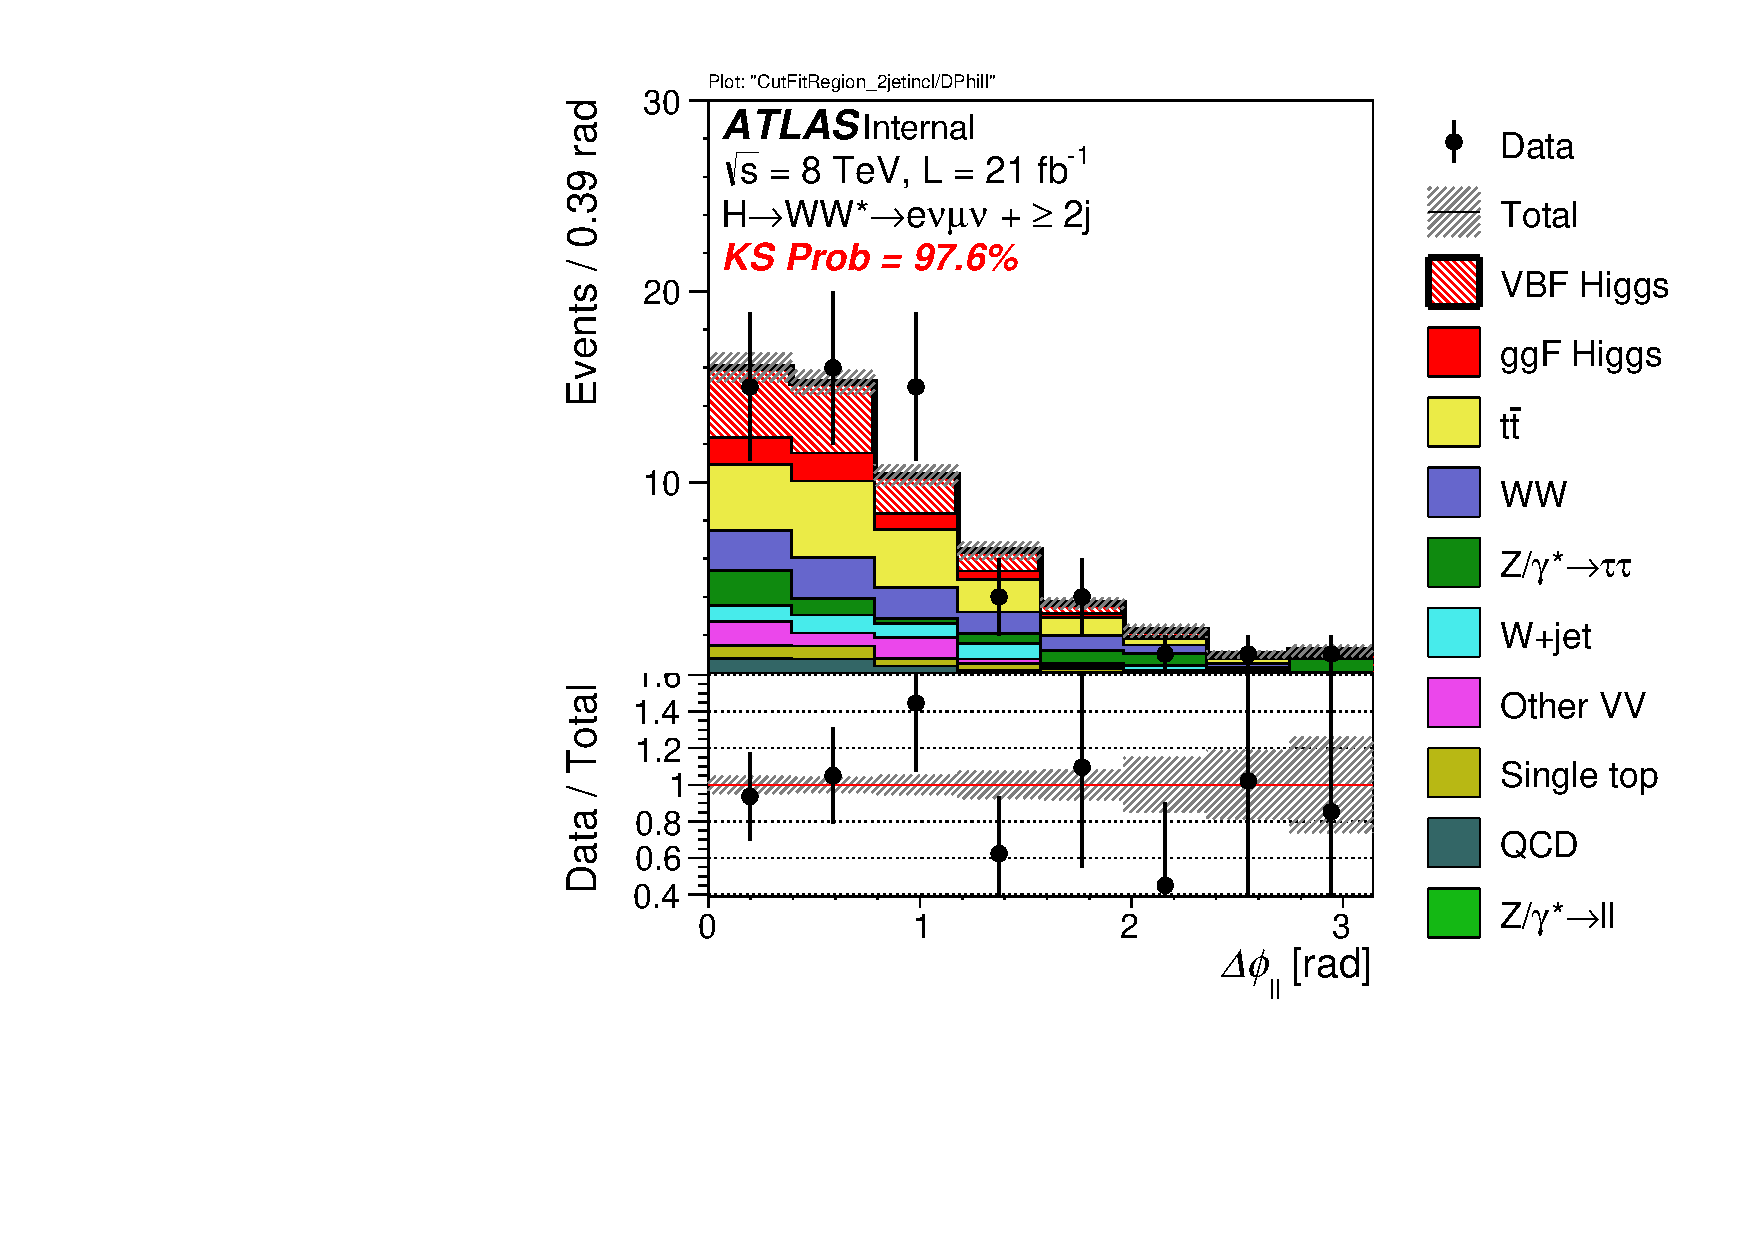
\includegraphics[width=0.4\textwidth]{fig/analysis/BDTinputVarsInSR/DF_SR_FitRegion_DPhill_mh125_lin.pdf}
   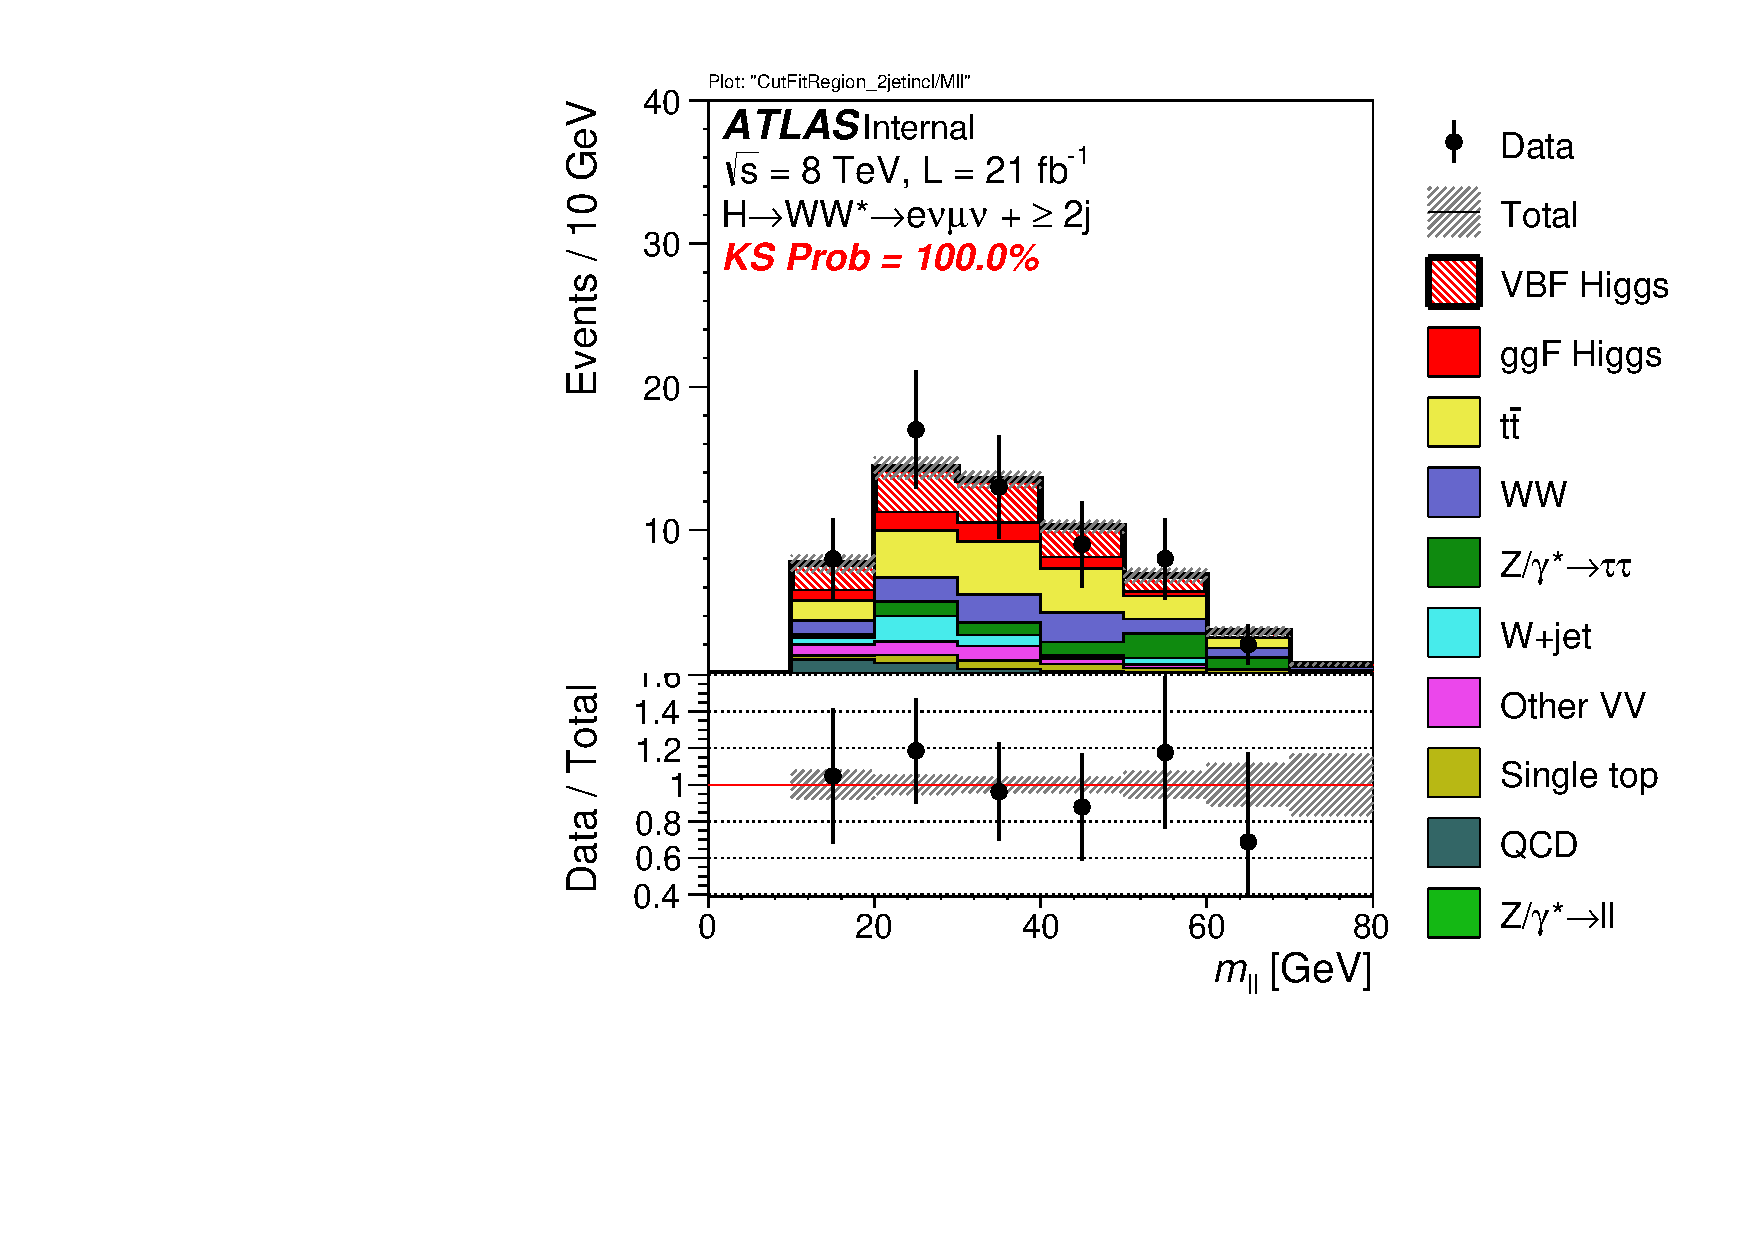
\includegraphics[width=0.4\textwidth]{fig/analysis/BDTinputVarsInSR/DF_SR_FitRegion_Mll_mh125_lin.pdf}
   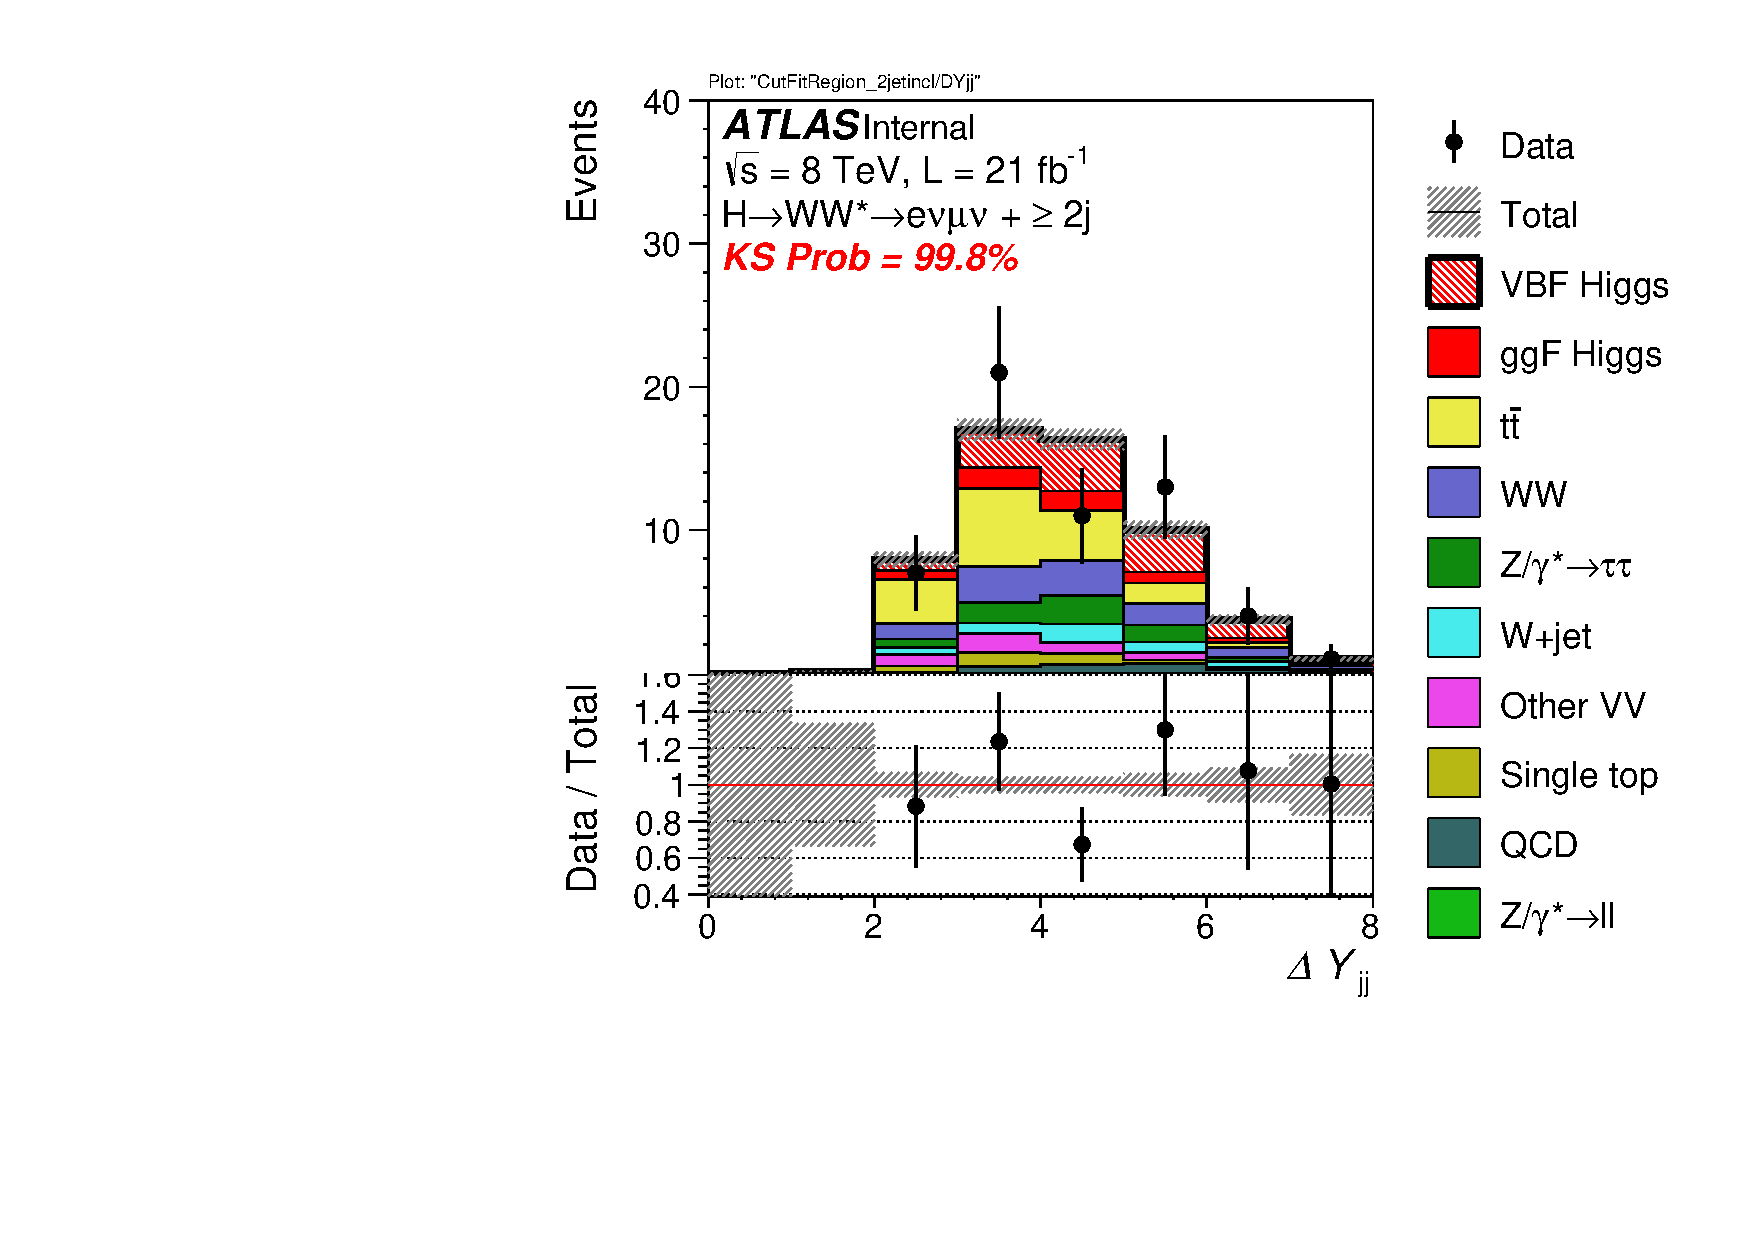
\includegraphics[width=0.4\textwidth]{fig/analysis/BDTinputVarsInSR/DF_SR_FitRegion_DYjj_mh125_lin.pdf}
   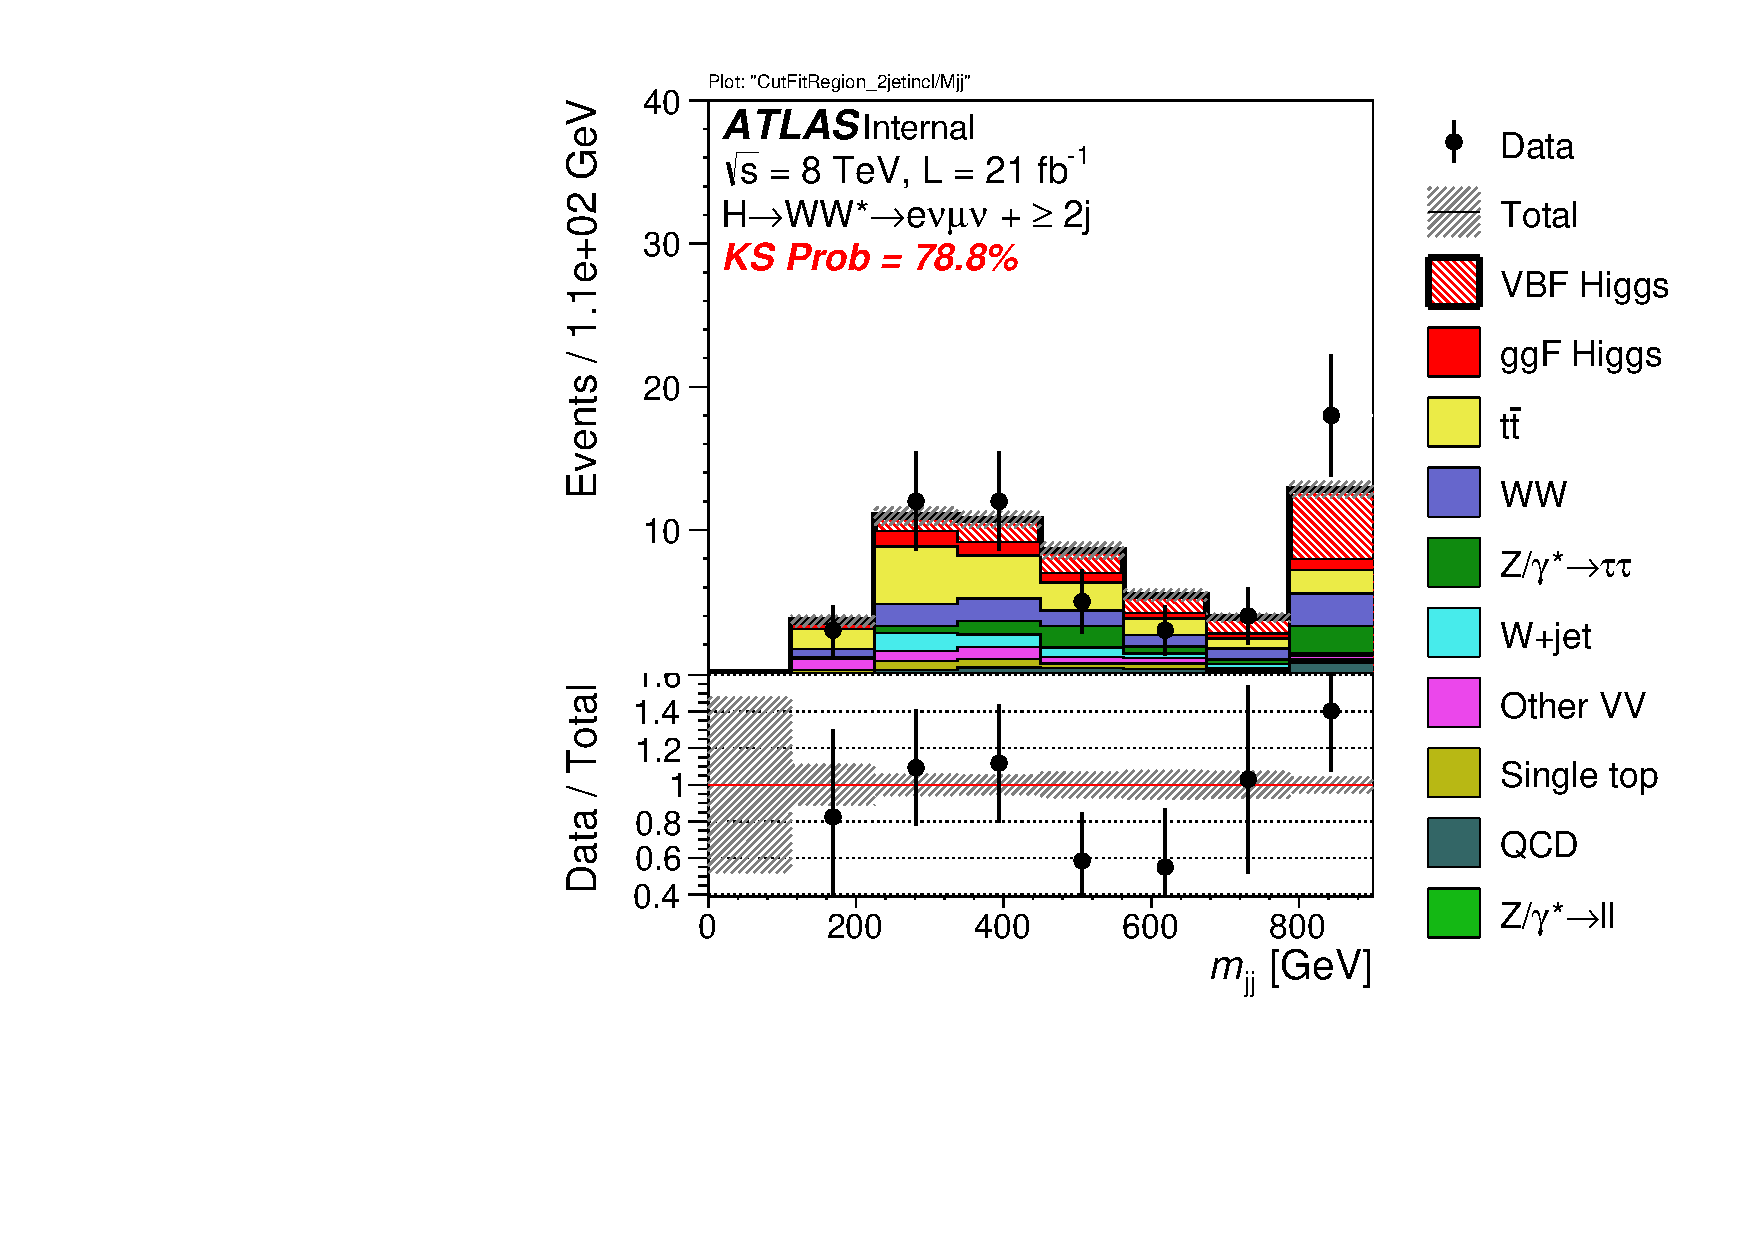
\includegraphics[width=0.4\textwidth]{fig/analysis/BDTinputVarsInSR/DF_SR_FitRegion_Mjj_mh125_lin.pdf}
   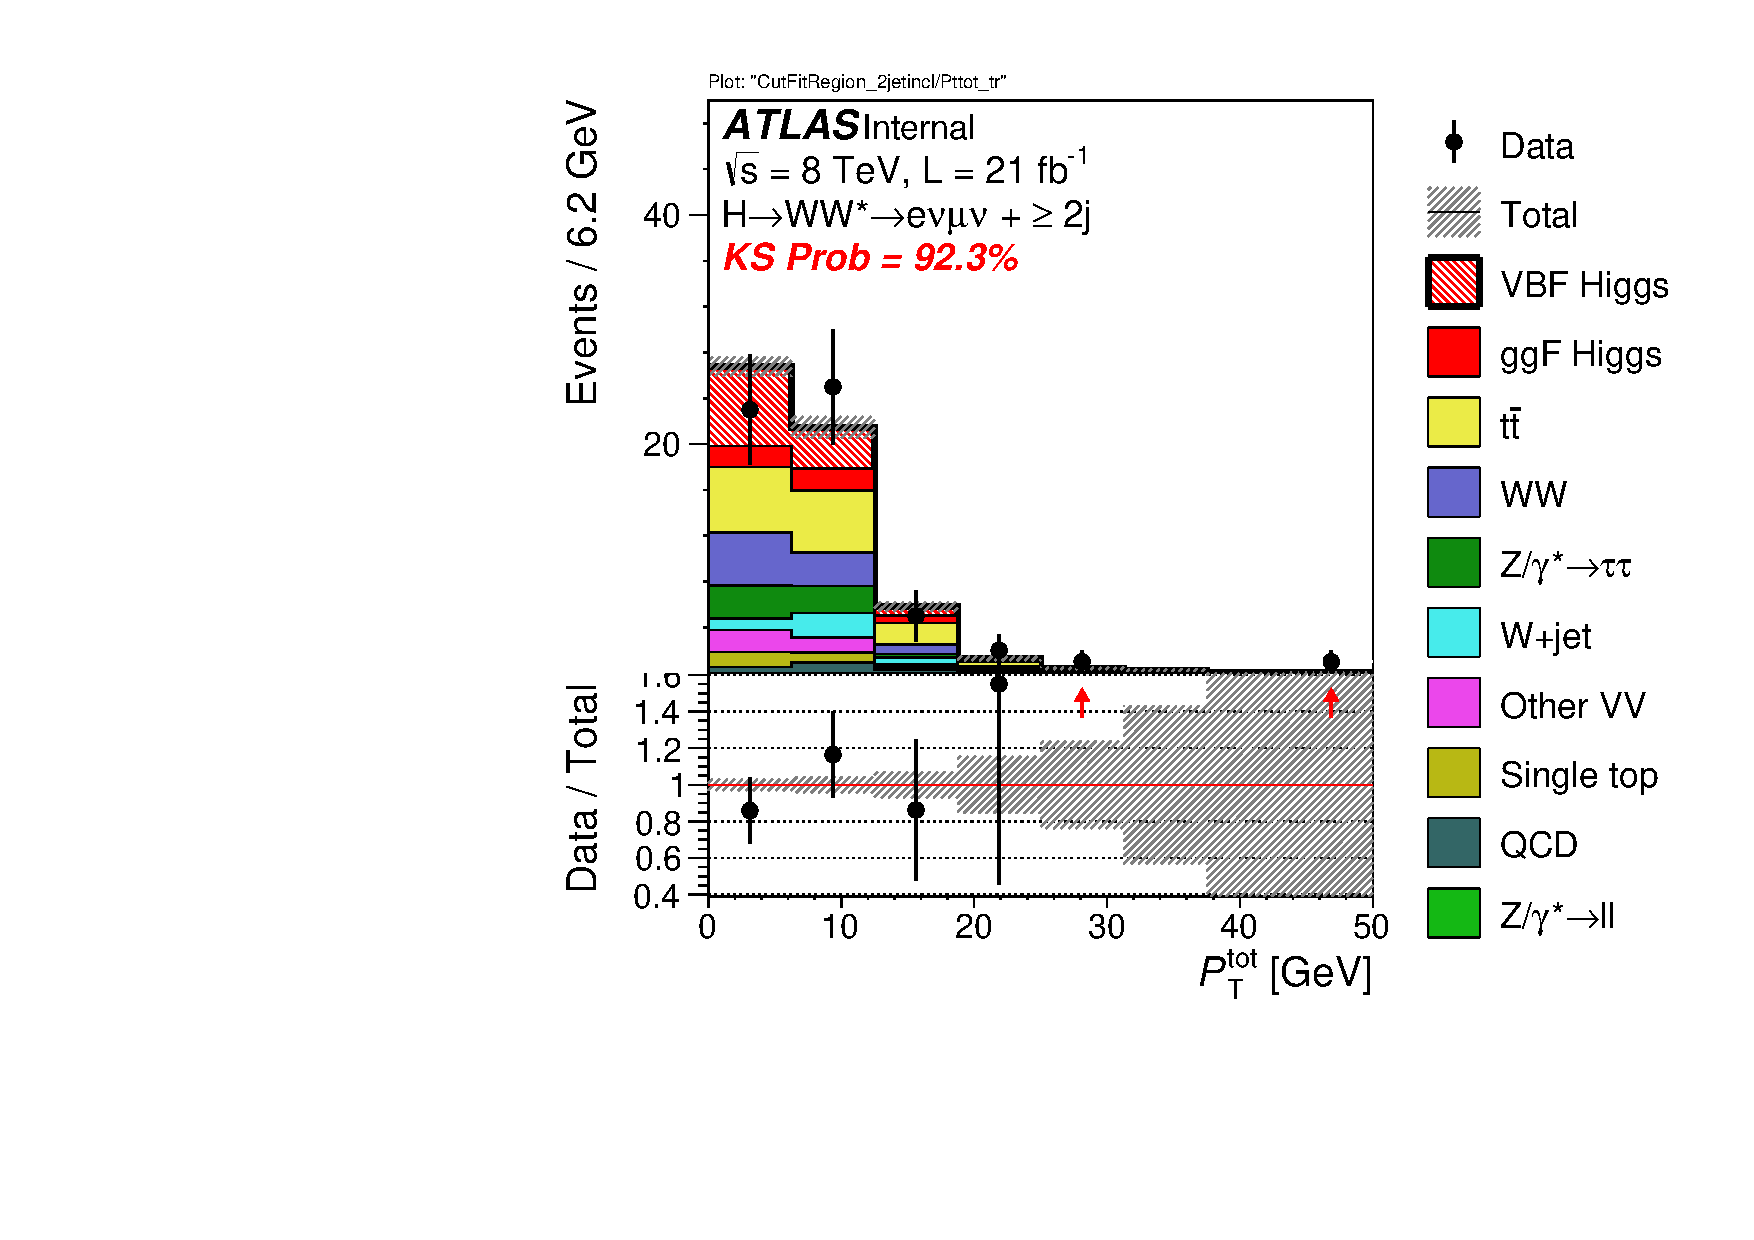
\includegraphics[width=0.4\textwidth]{fig/analysis/BDTinputVarsInSR/DF_SR_FitRegion_Pttot_tr_mh125_lin.pdf}
   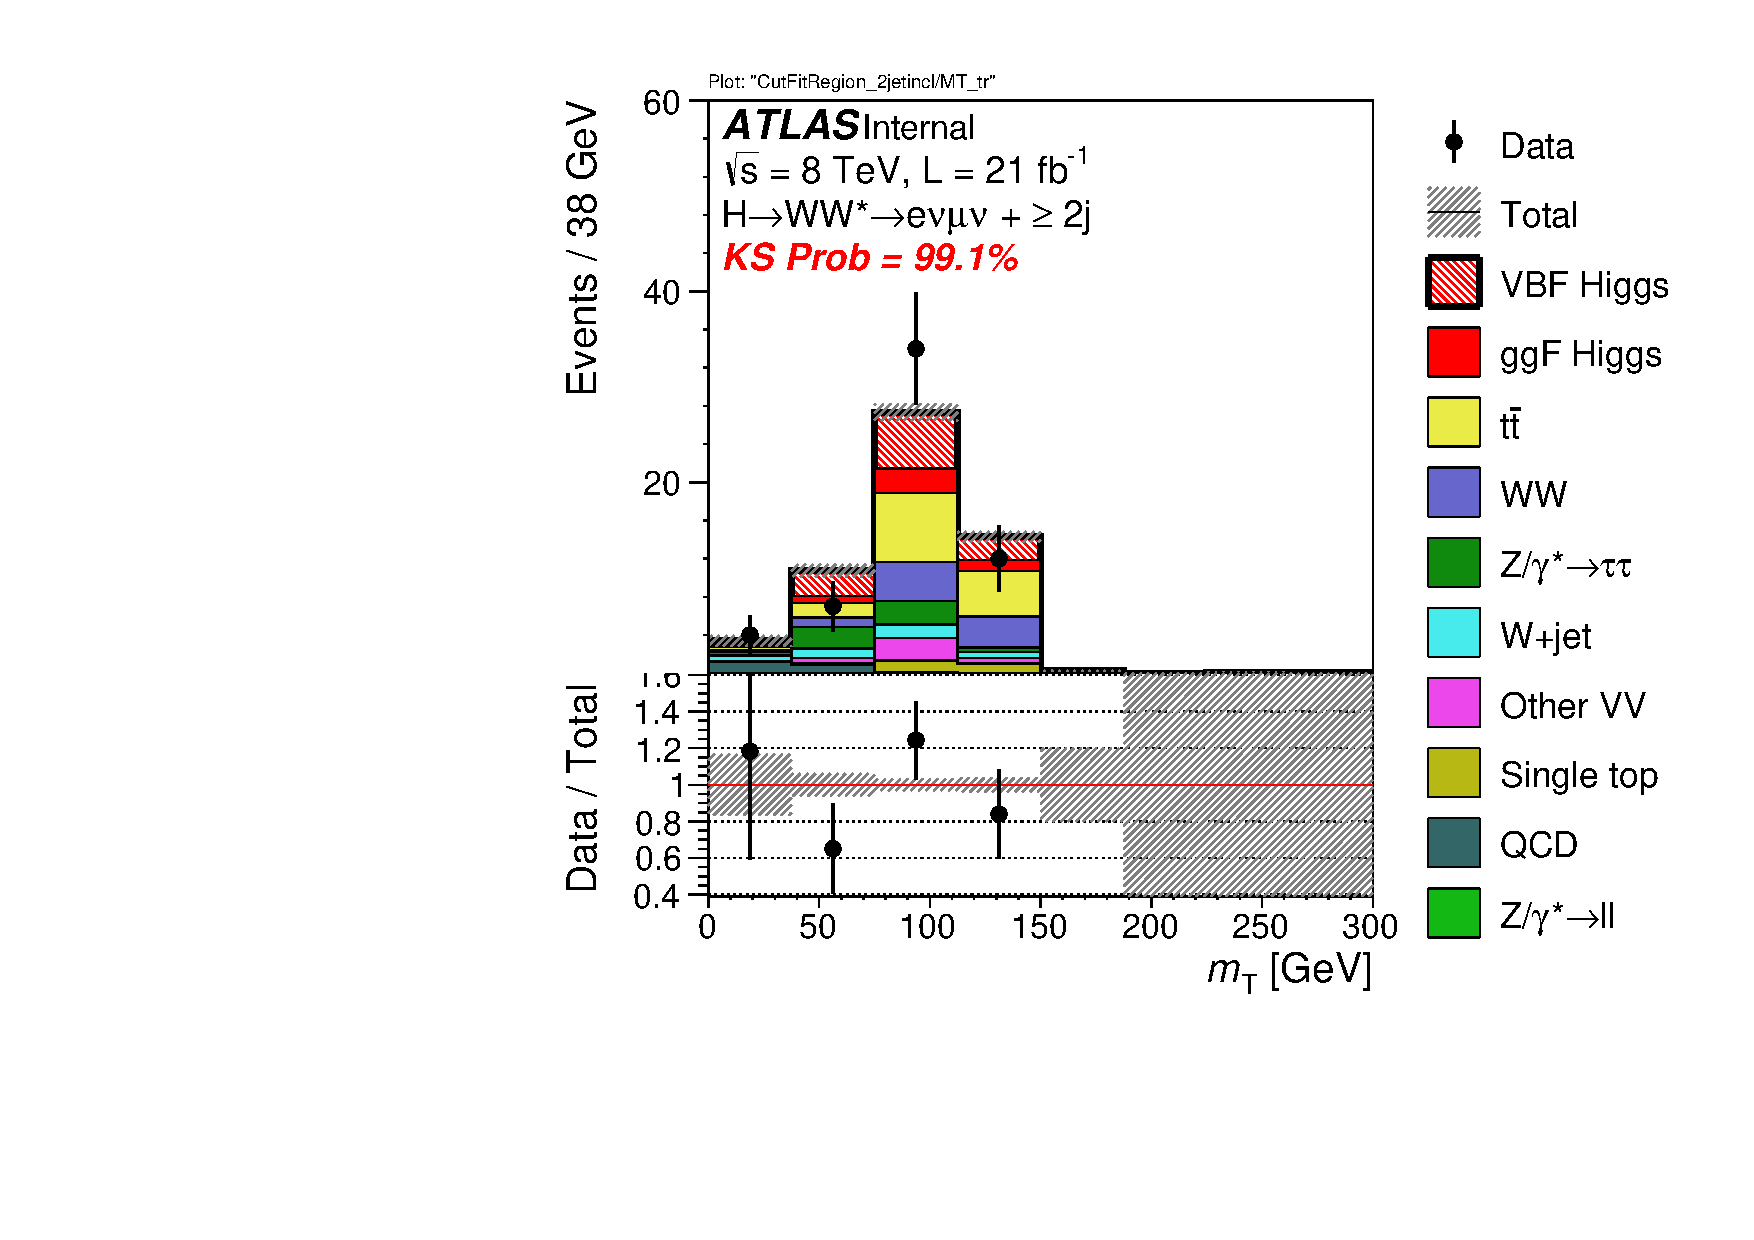
\includegraphics[width=0.4\textwidth]{fig/analysis/BDTinputVarsInSR/DF_SR_FitRegion_MT_tr_mh125_lin.pdf}
   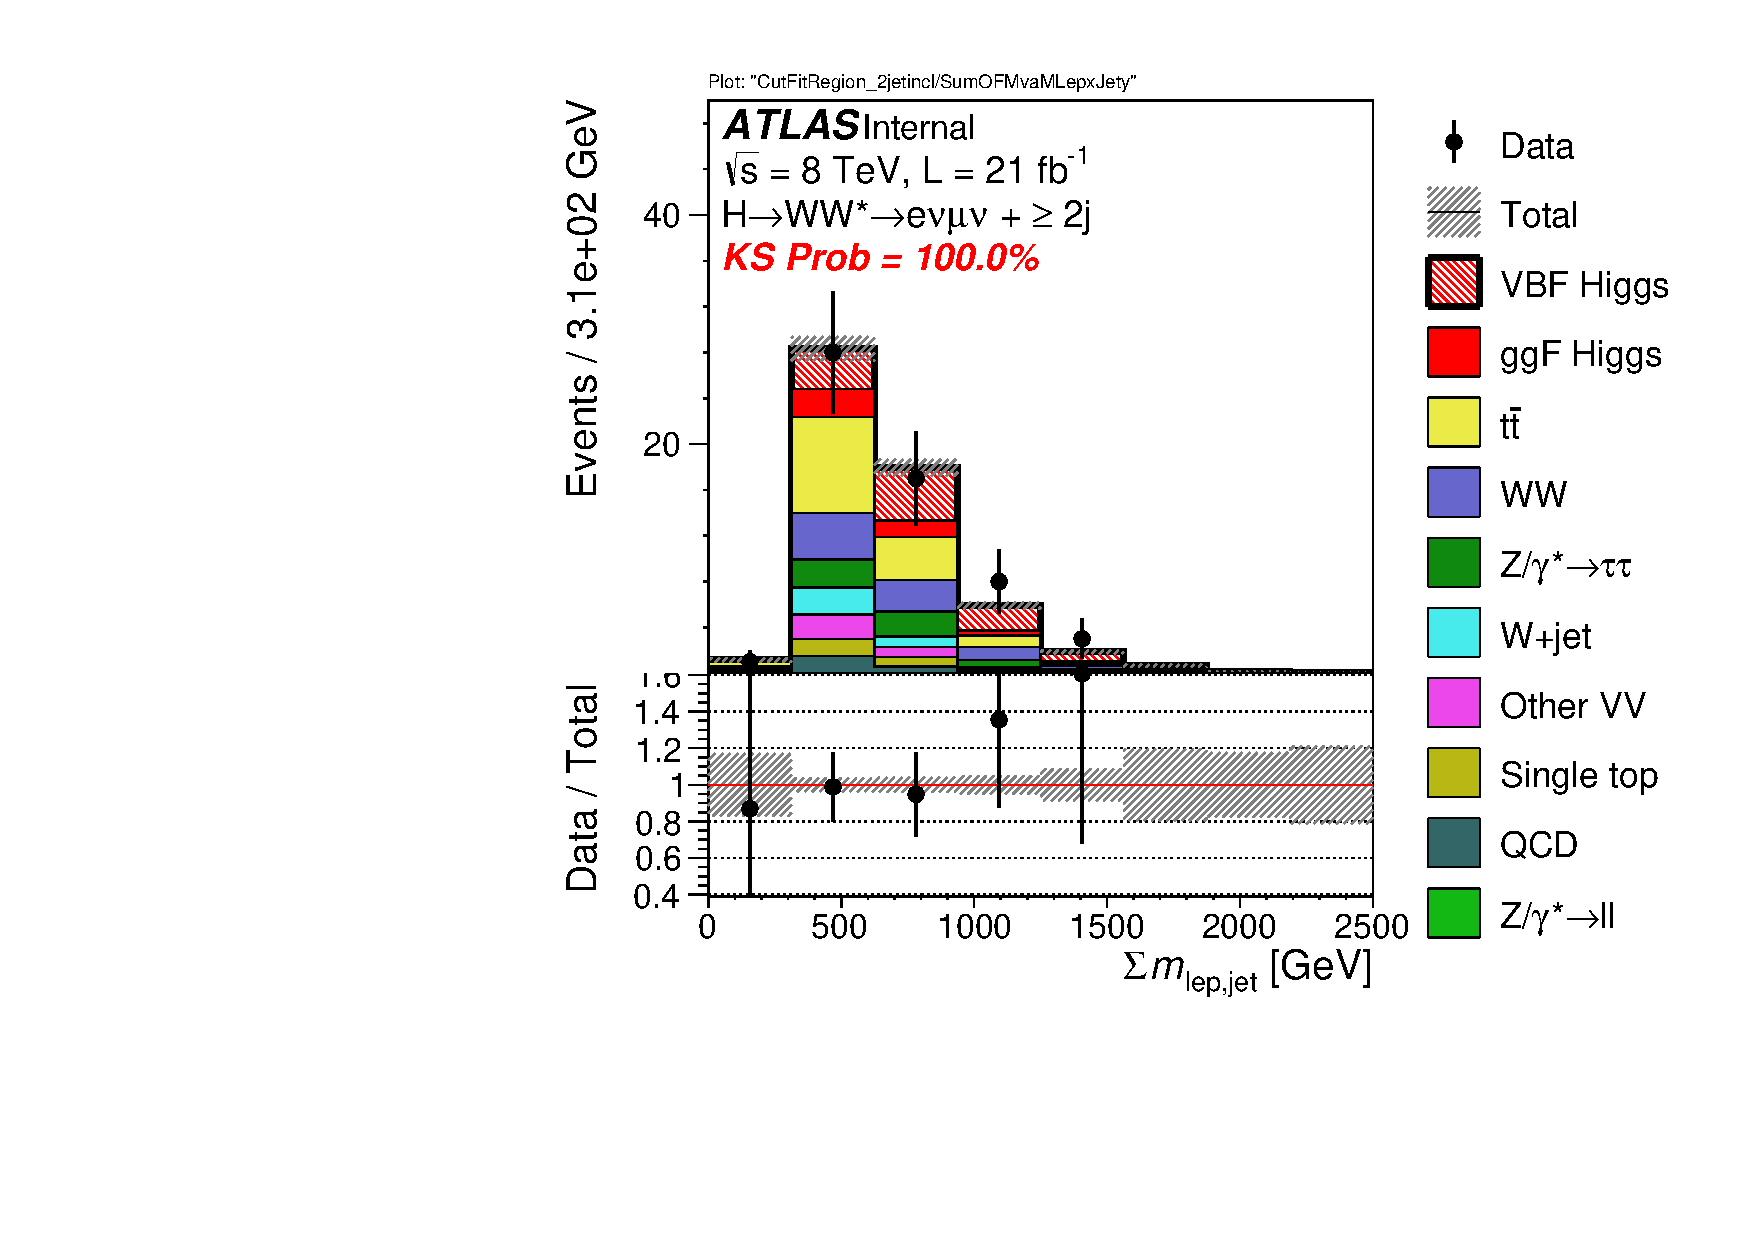
\includegraphics[width=0.4\textwidth]{fig/analysis/BDTinputVarsInSR/DF_SR_FitRegion_SumOFMvaMLepxJety_mh125_lin.pdf}
   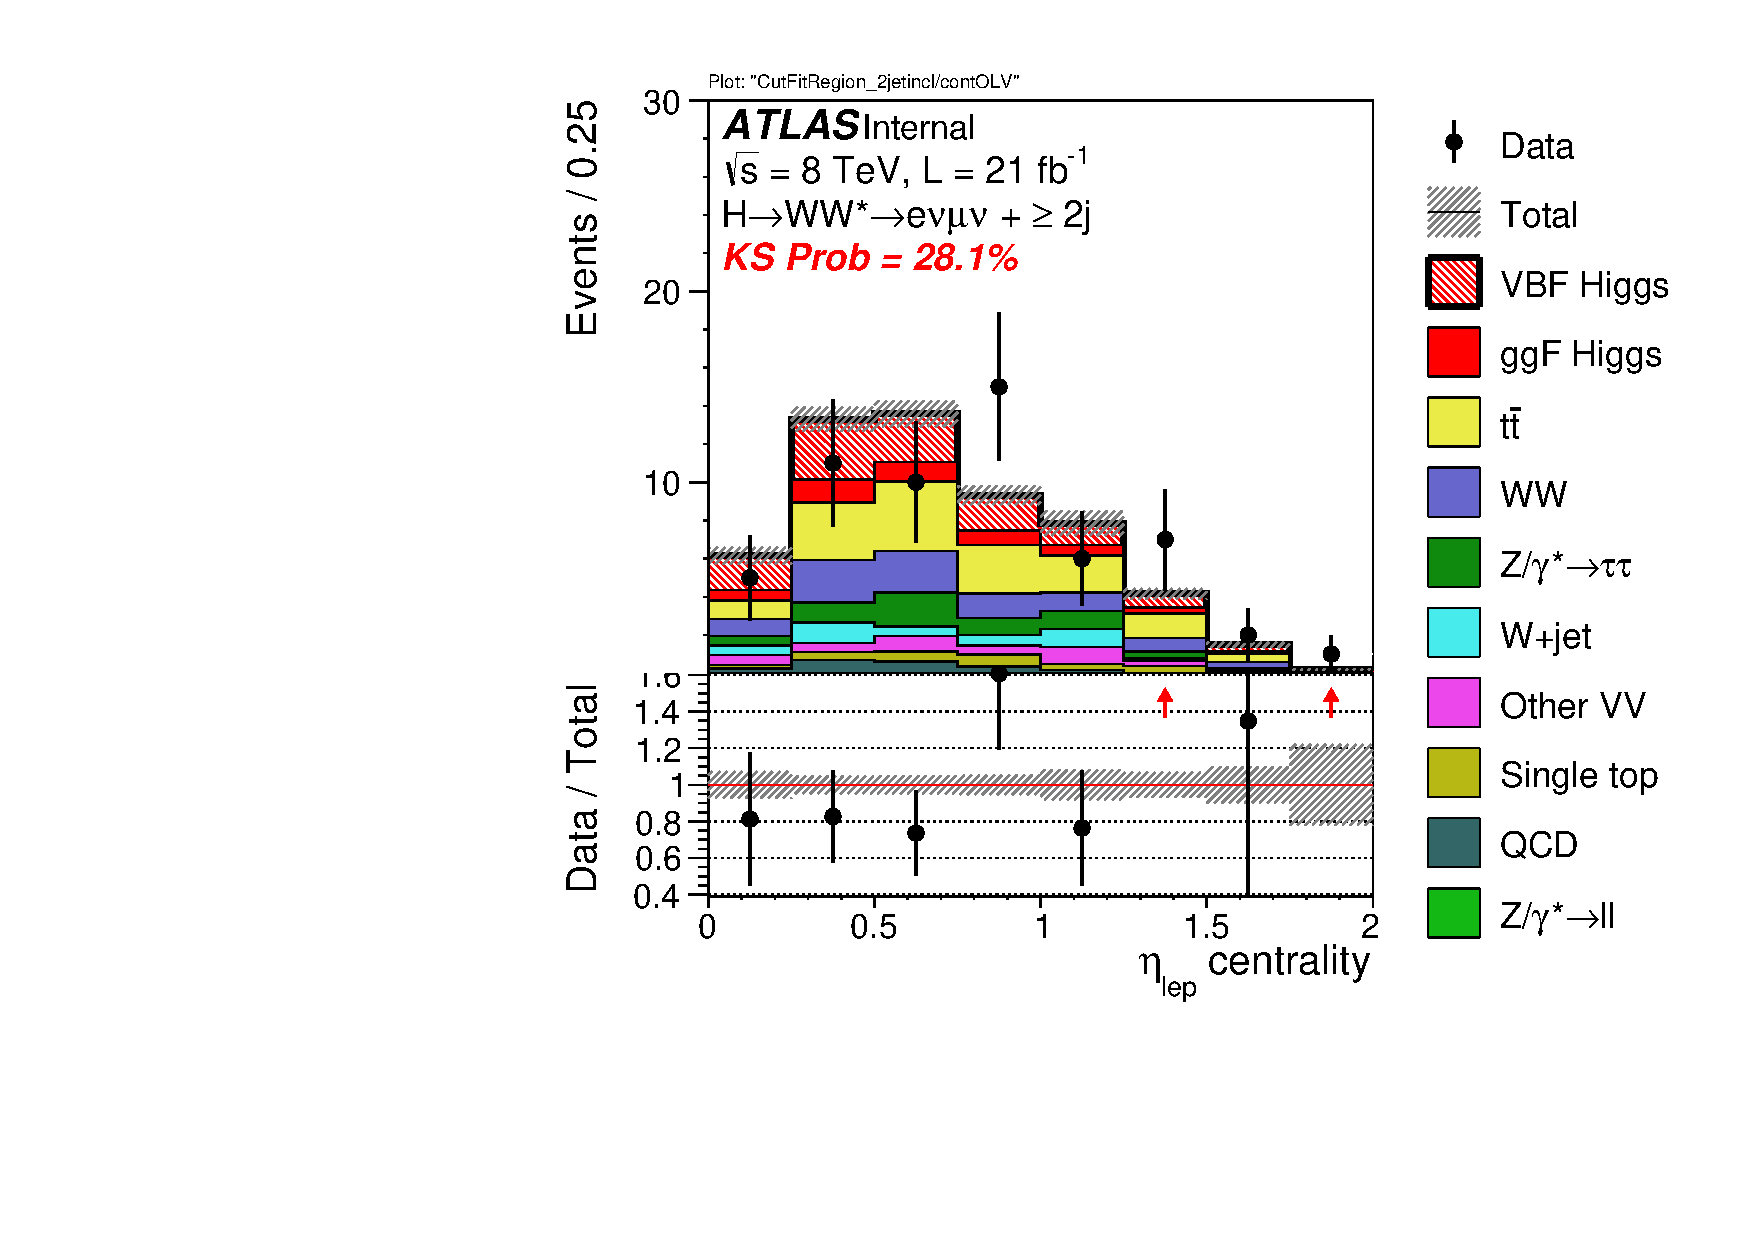
\includegraphics[width=0.4\textwidth]{fig/analysis/BDTinputVarsInSR/DF_SR_FitRegion_contOLV_mh125_lin.pdf}
   \caption{Distributions
   of \dphill, \mll, \dyjj, \mjj, \pTtot, \mT, \SumMlj, and
   \lepEtaCent
   in the \emme channel in the high BDT fit region ($\textrm{BDT} > -0.48$).}
  \label{chap:analysis:fig:bdt_inputs_sr_df}
\end{figure}

\begin{figure}[hb!]
  \centering
   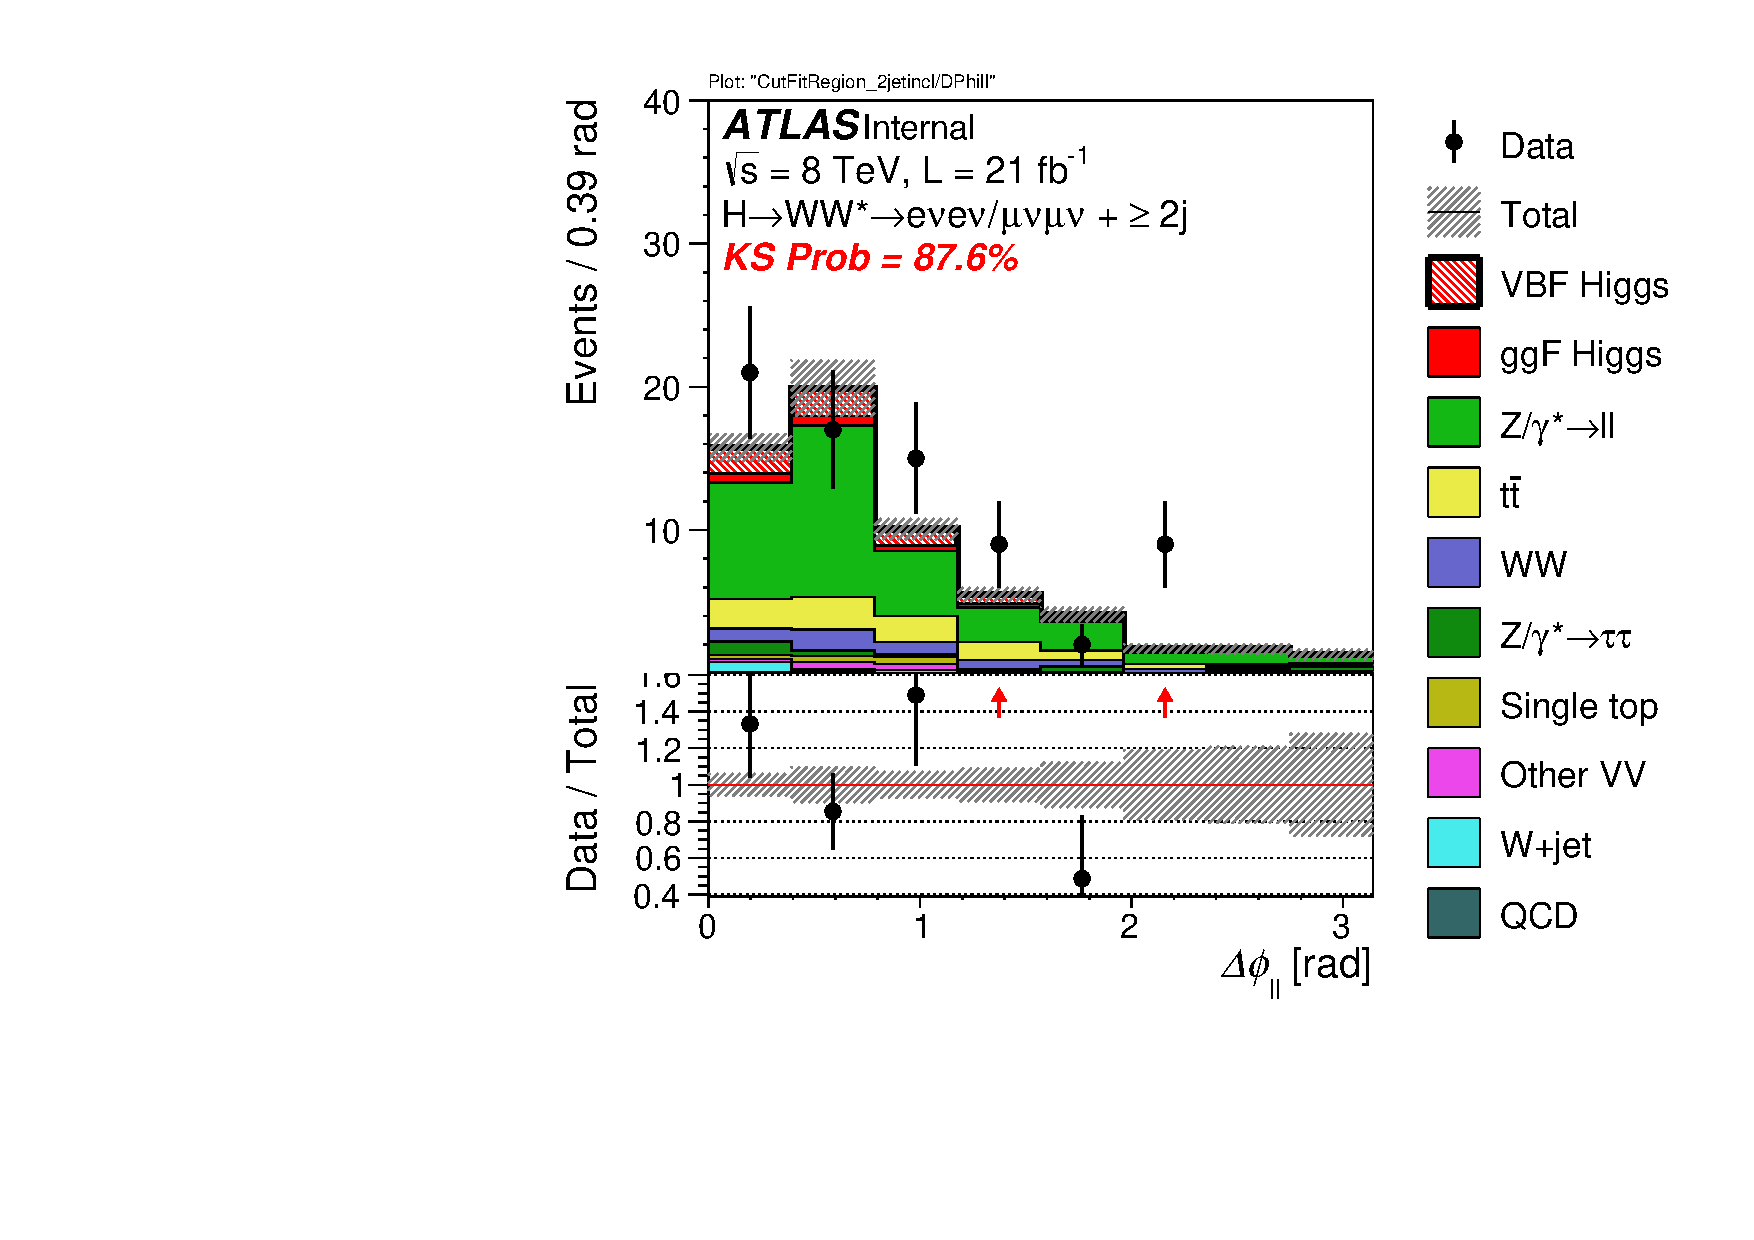
\includegraphics[width=0.4\textwidth]{fig/analysis/BDTinputVarsInSR/SF_SR_FitRegion_DPhill_mh125_lin.pdf}
   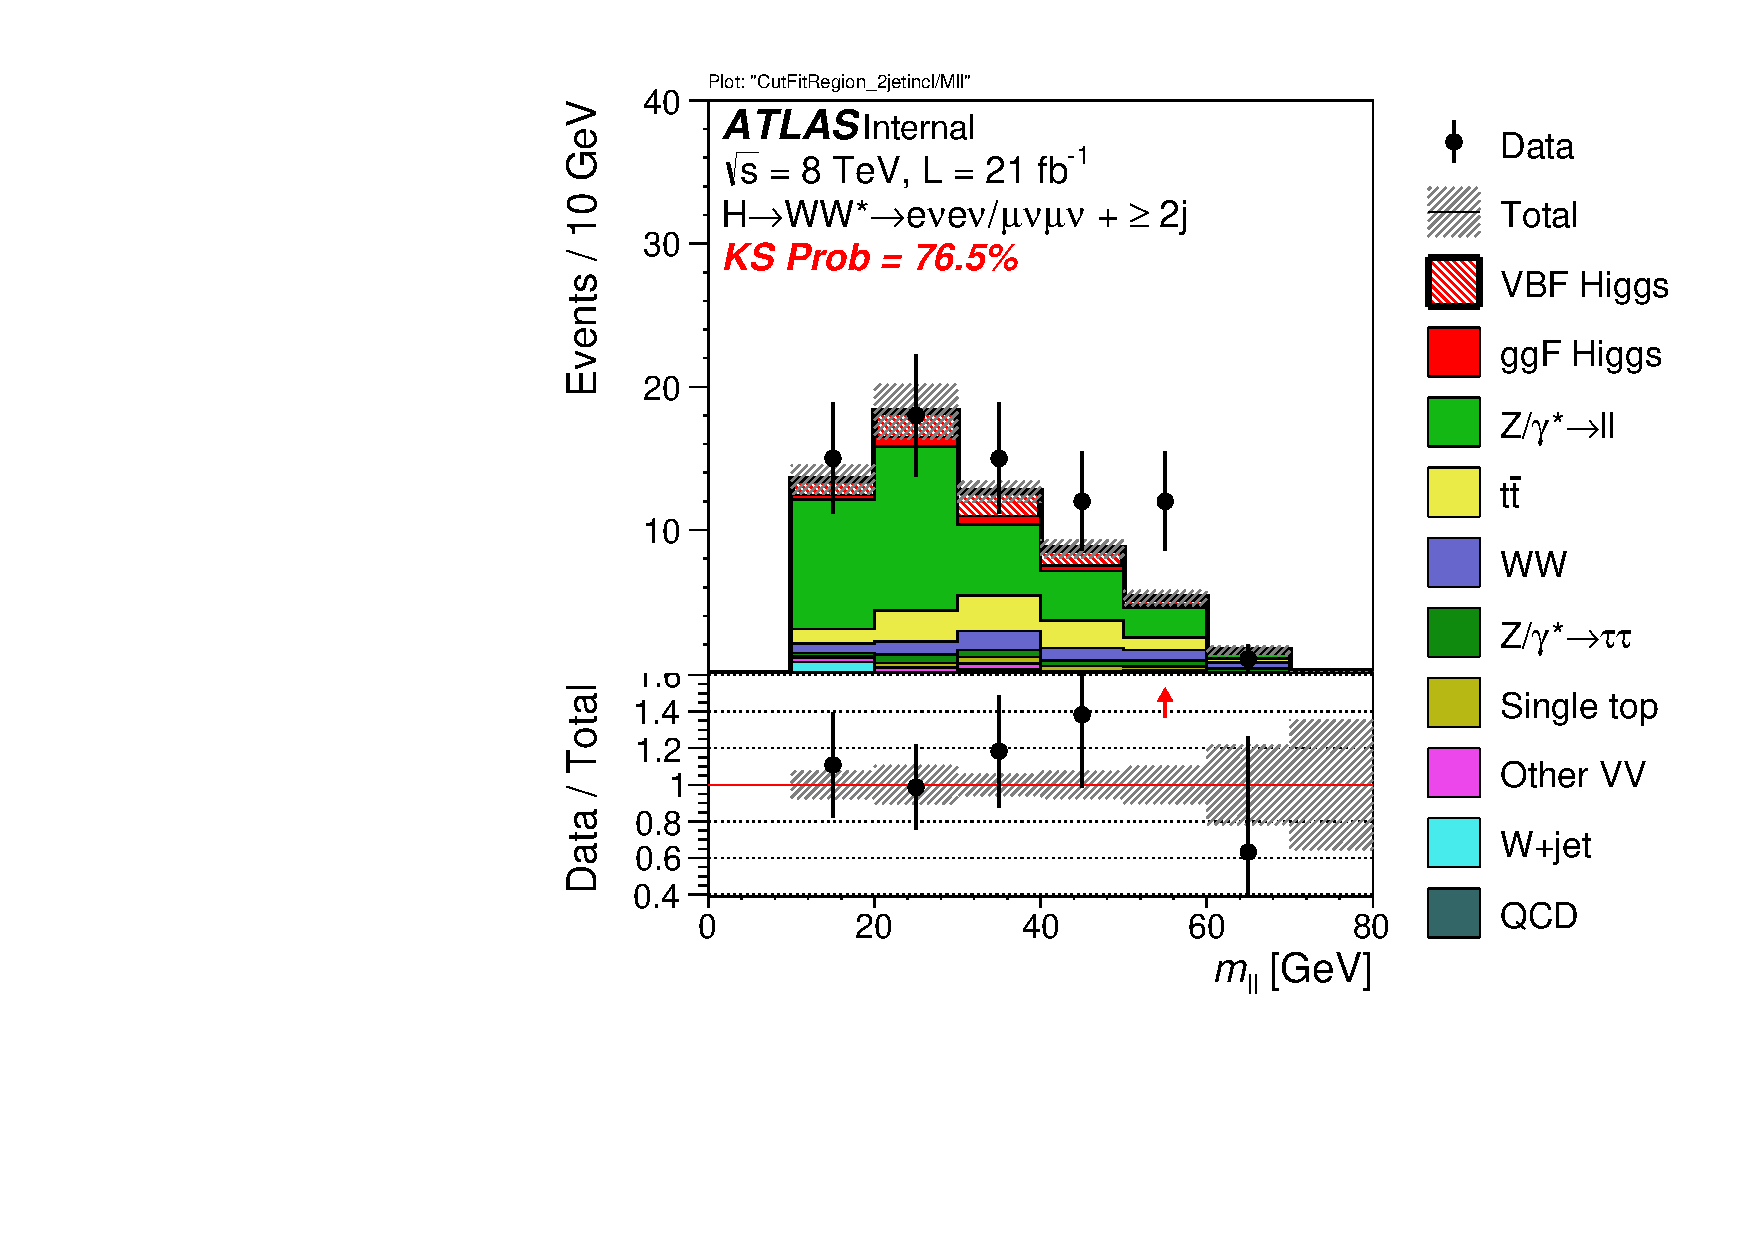
\includegraphics[width=0.4\textwidth]{fig/analysis/BDTinputVarsInSR/SF_SR_FitRegion_Mll_mh125_lin.pdf}
   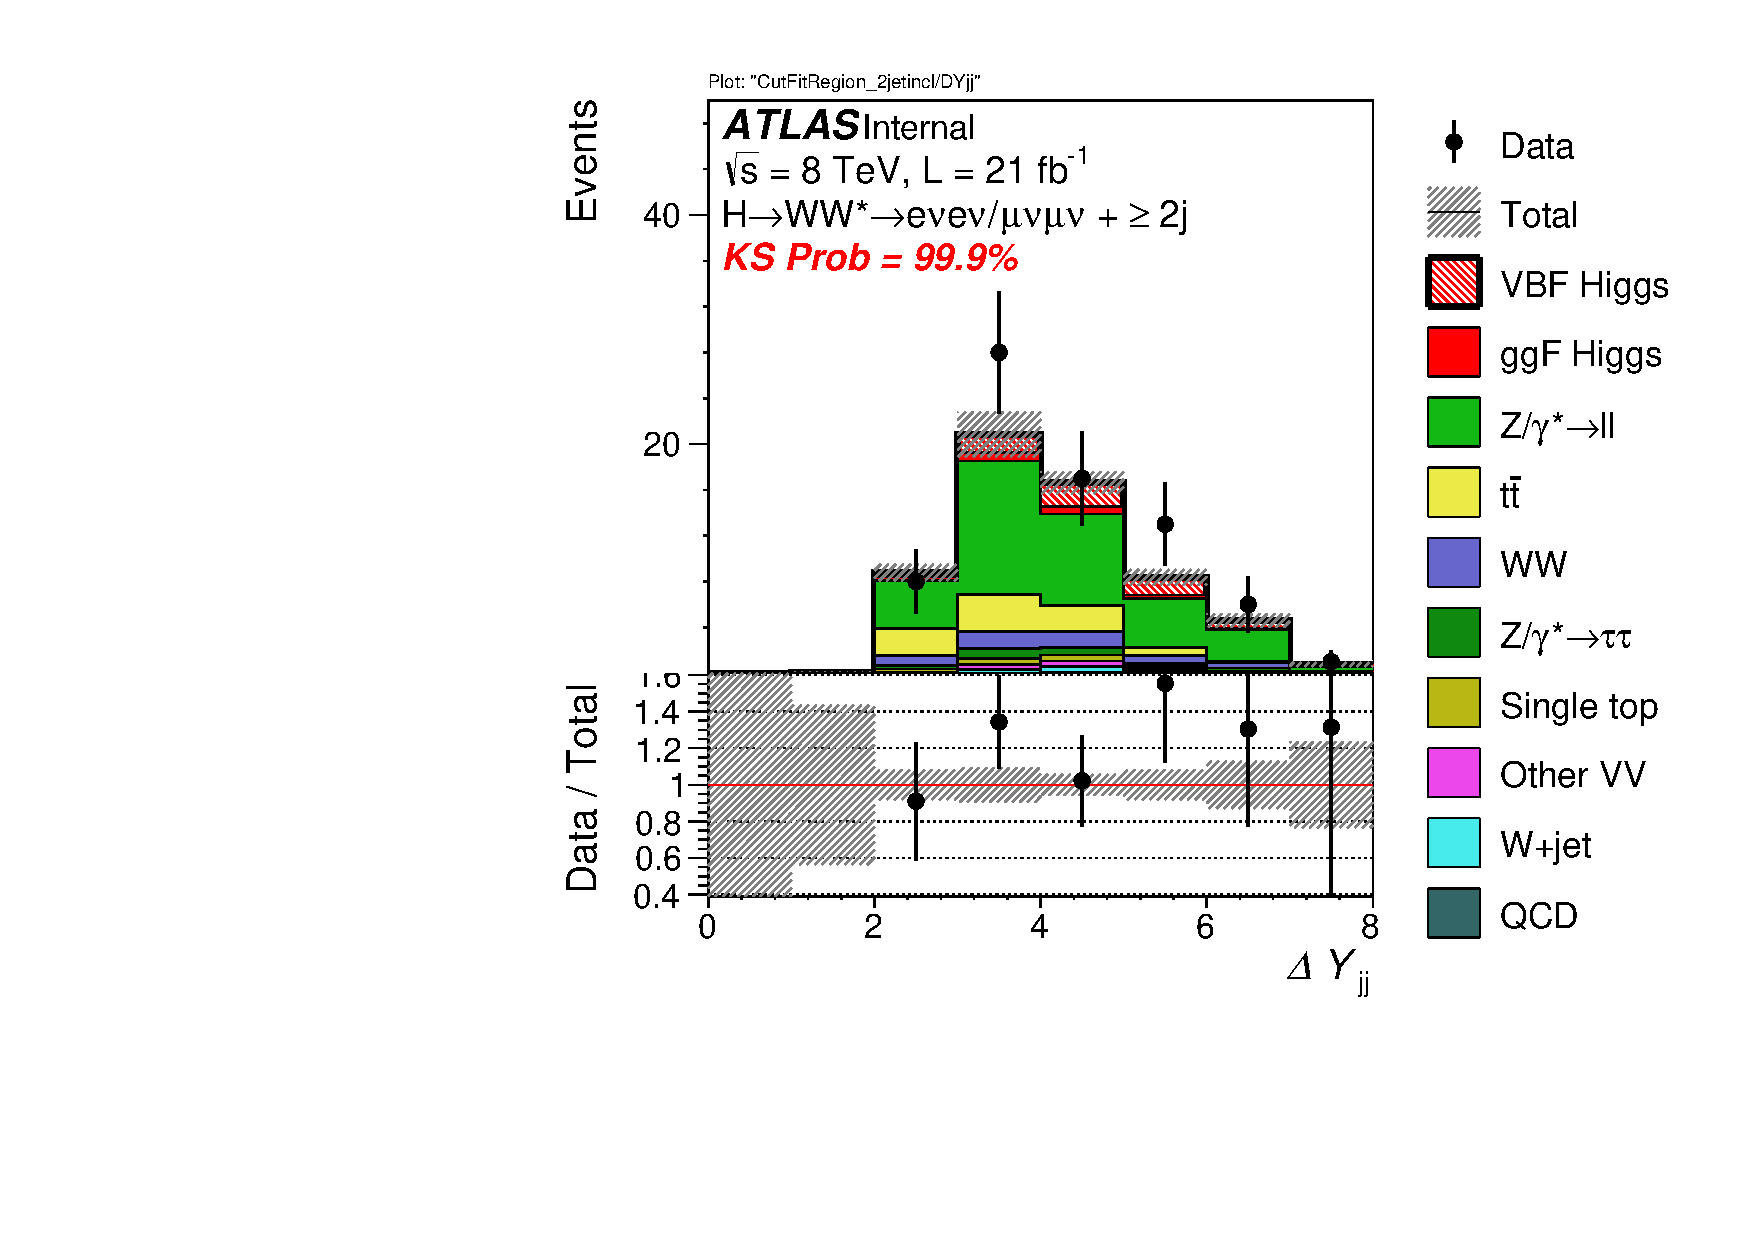
\includegraphics[width=0.4\textwidth]{fig/analysis/BDTinputVarsInSR/SF_SR_FitRegion_DYjj_mh125_lin.pdf}
   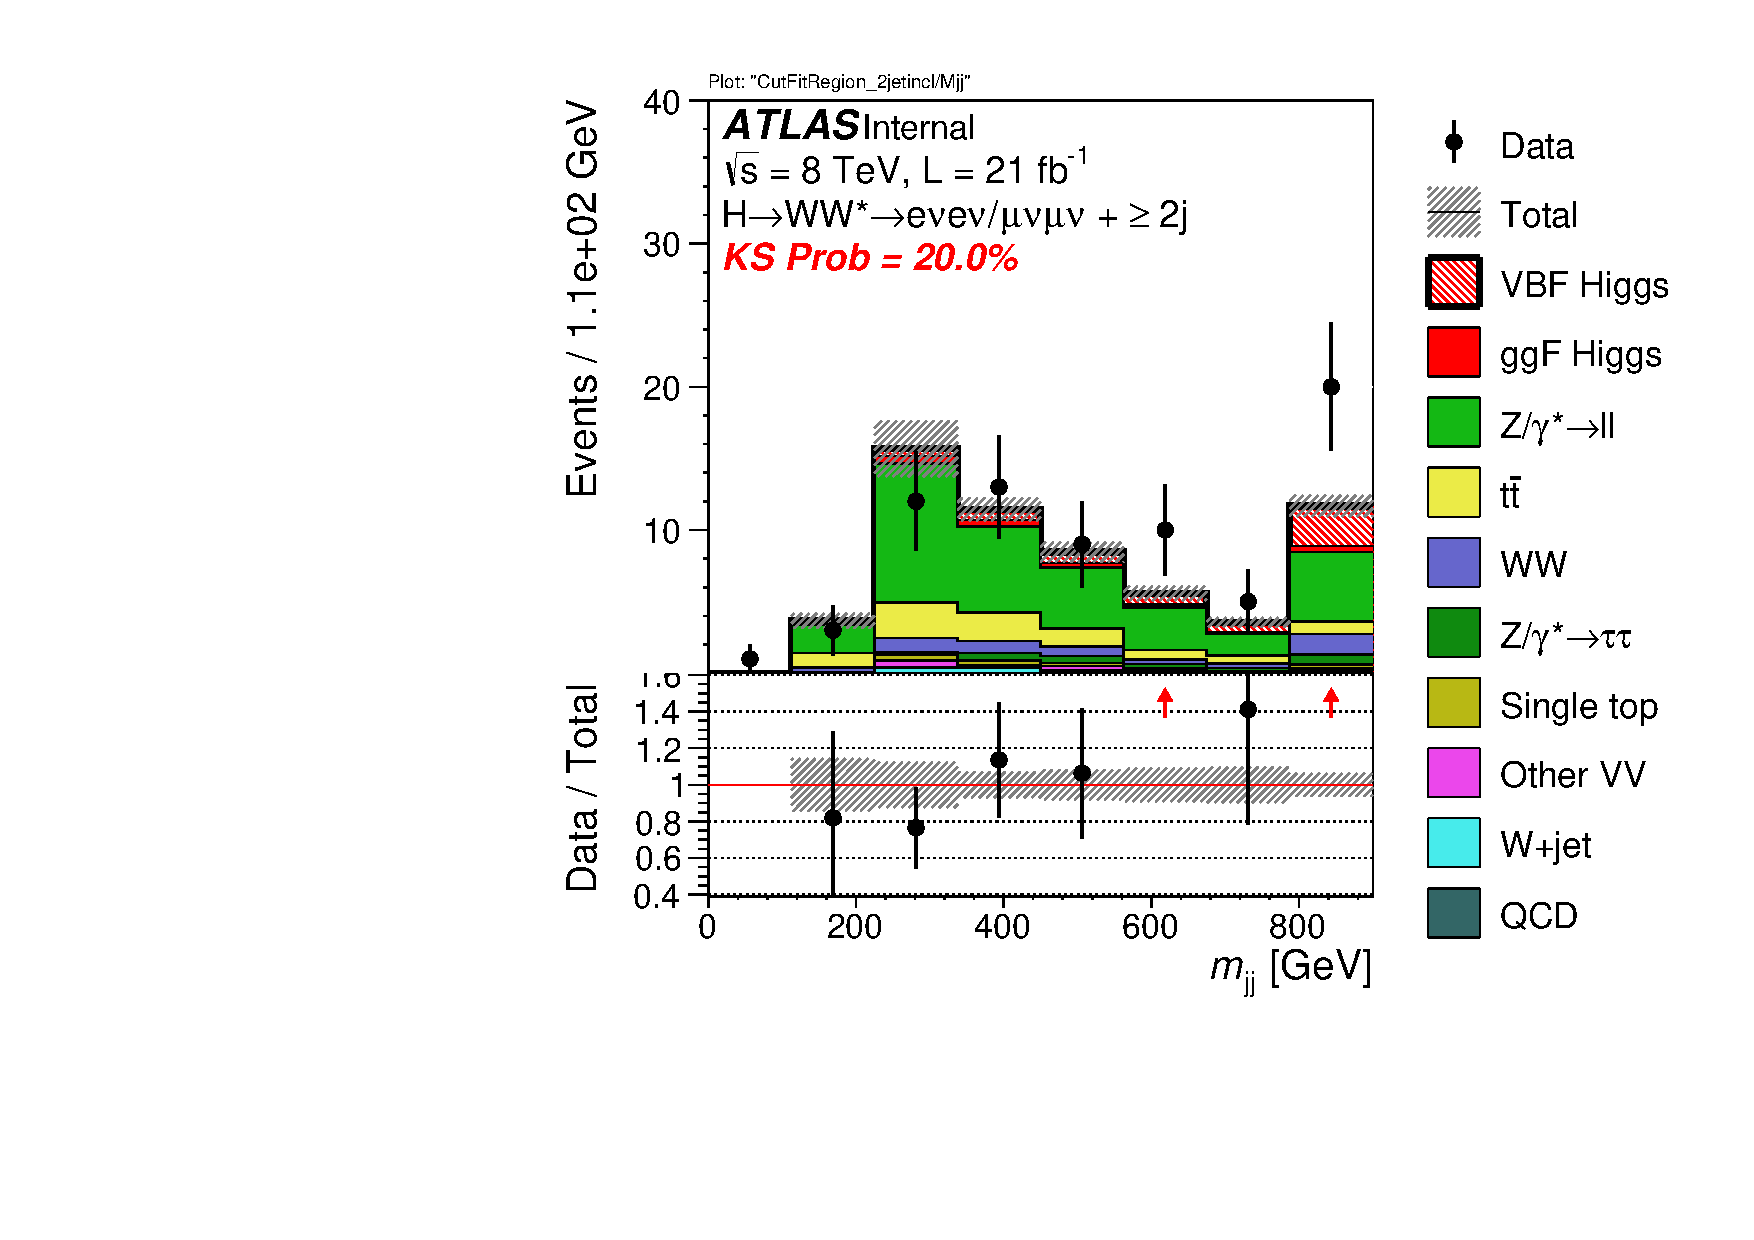
\includegraphics[width=0.4\textwidth]{fig/analysis/BDTinputVarsInSR/SF_SR_FitRegion_Mjj_mh125_lin.pdf}
   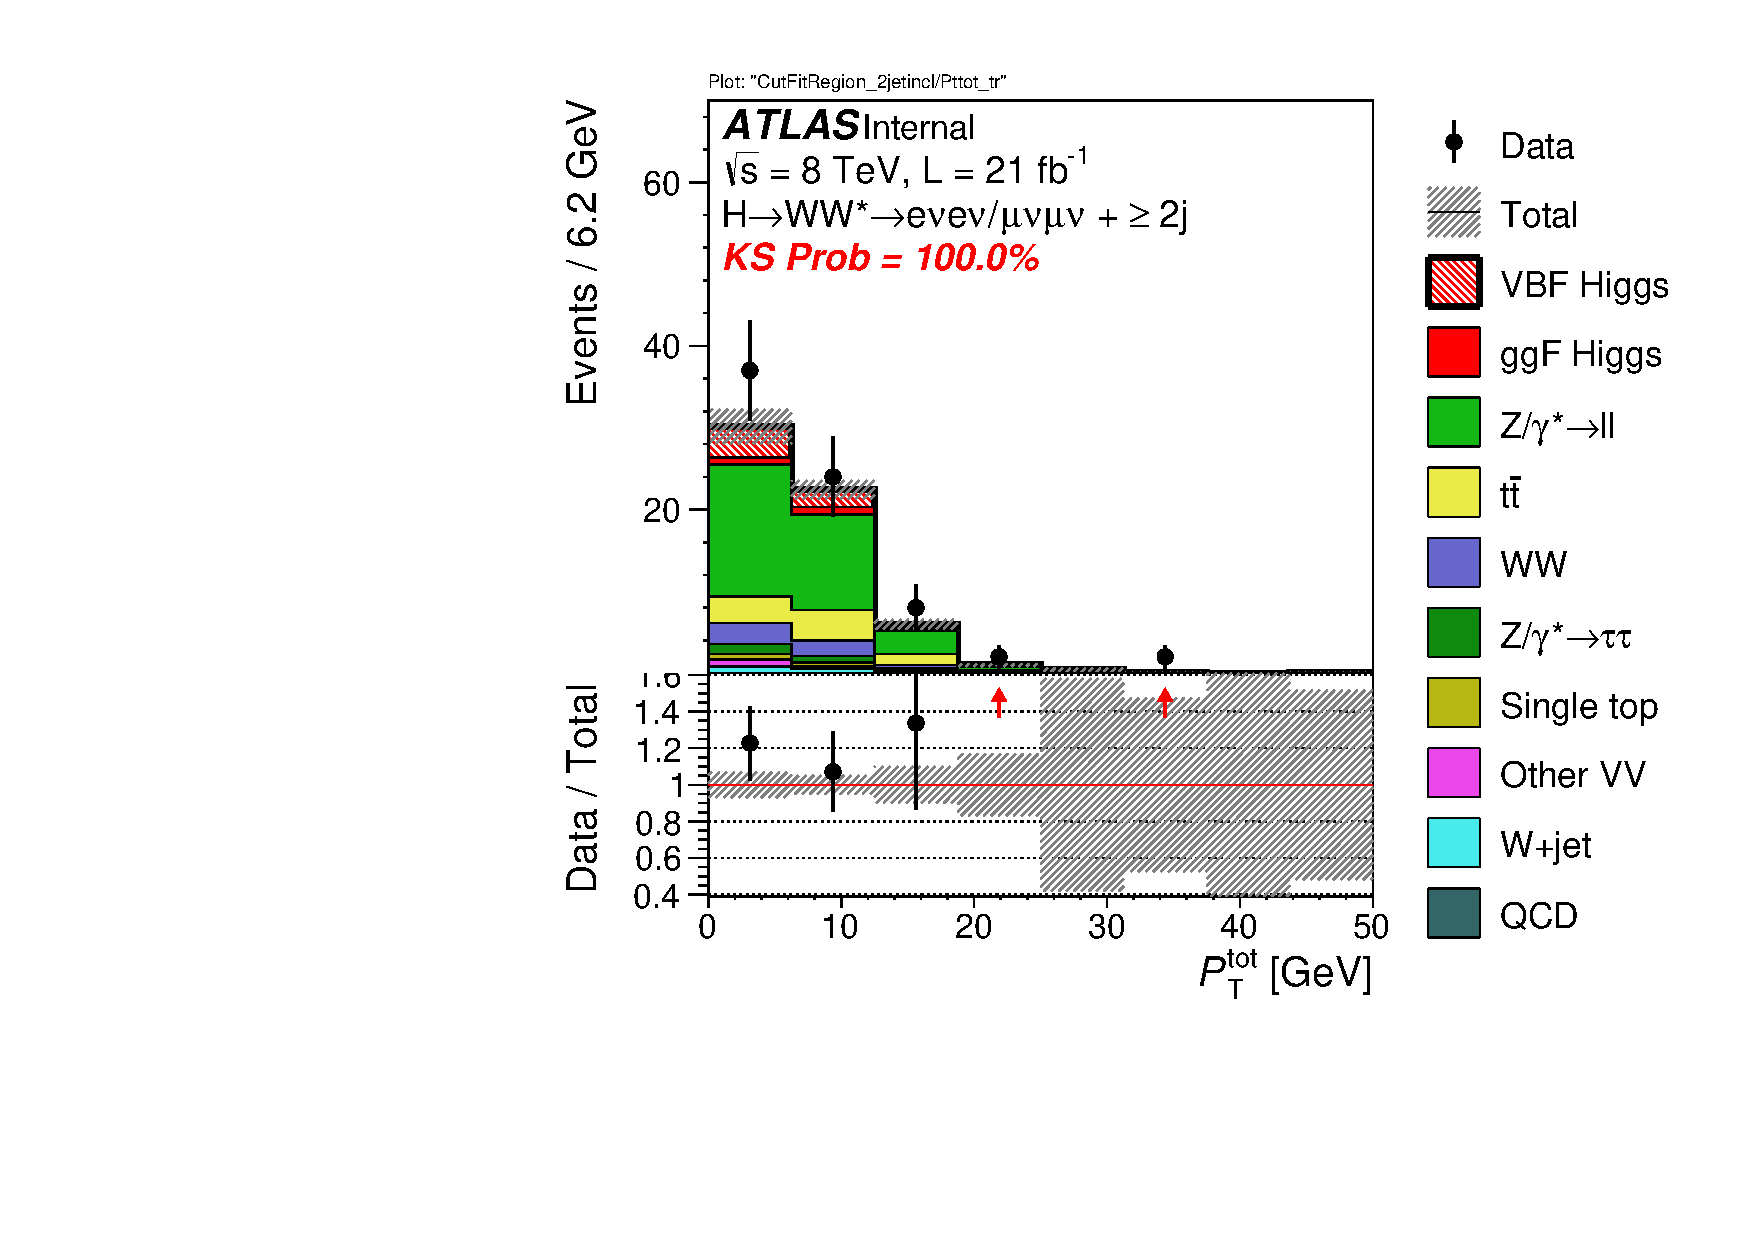
\includegraphics[width=0.4\textwidth]{fig/analysis/BDTinputVarsInSR/SF_SR_FitRegion_Pttot_tr_mh125_lin.pdf}
   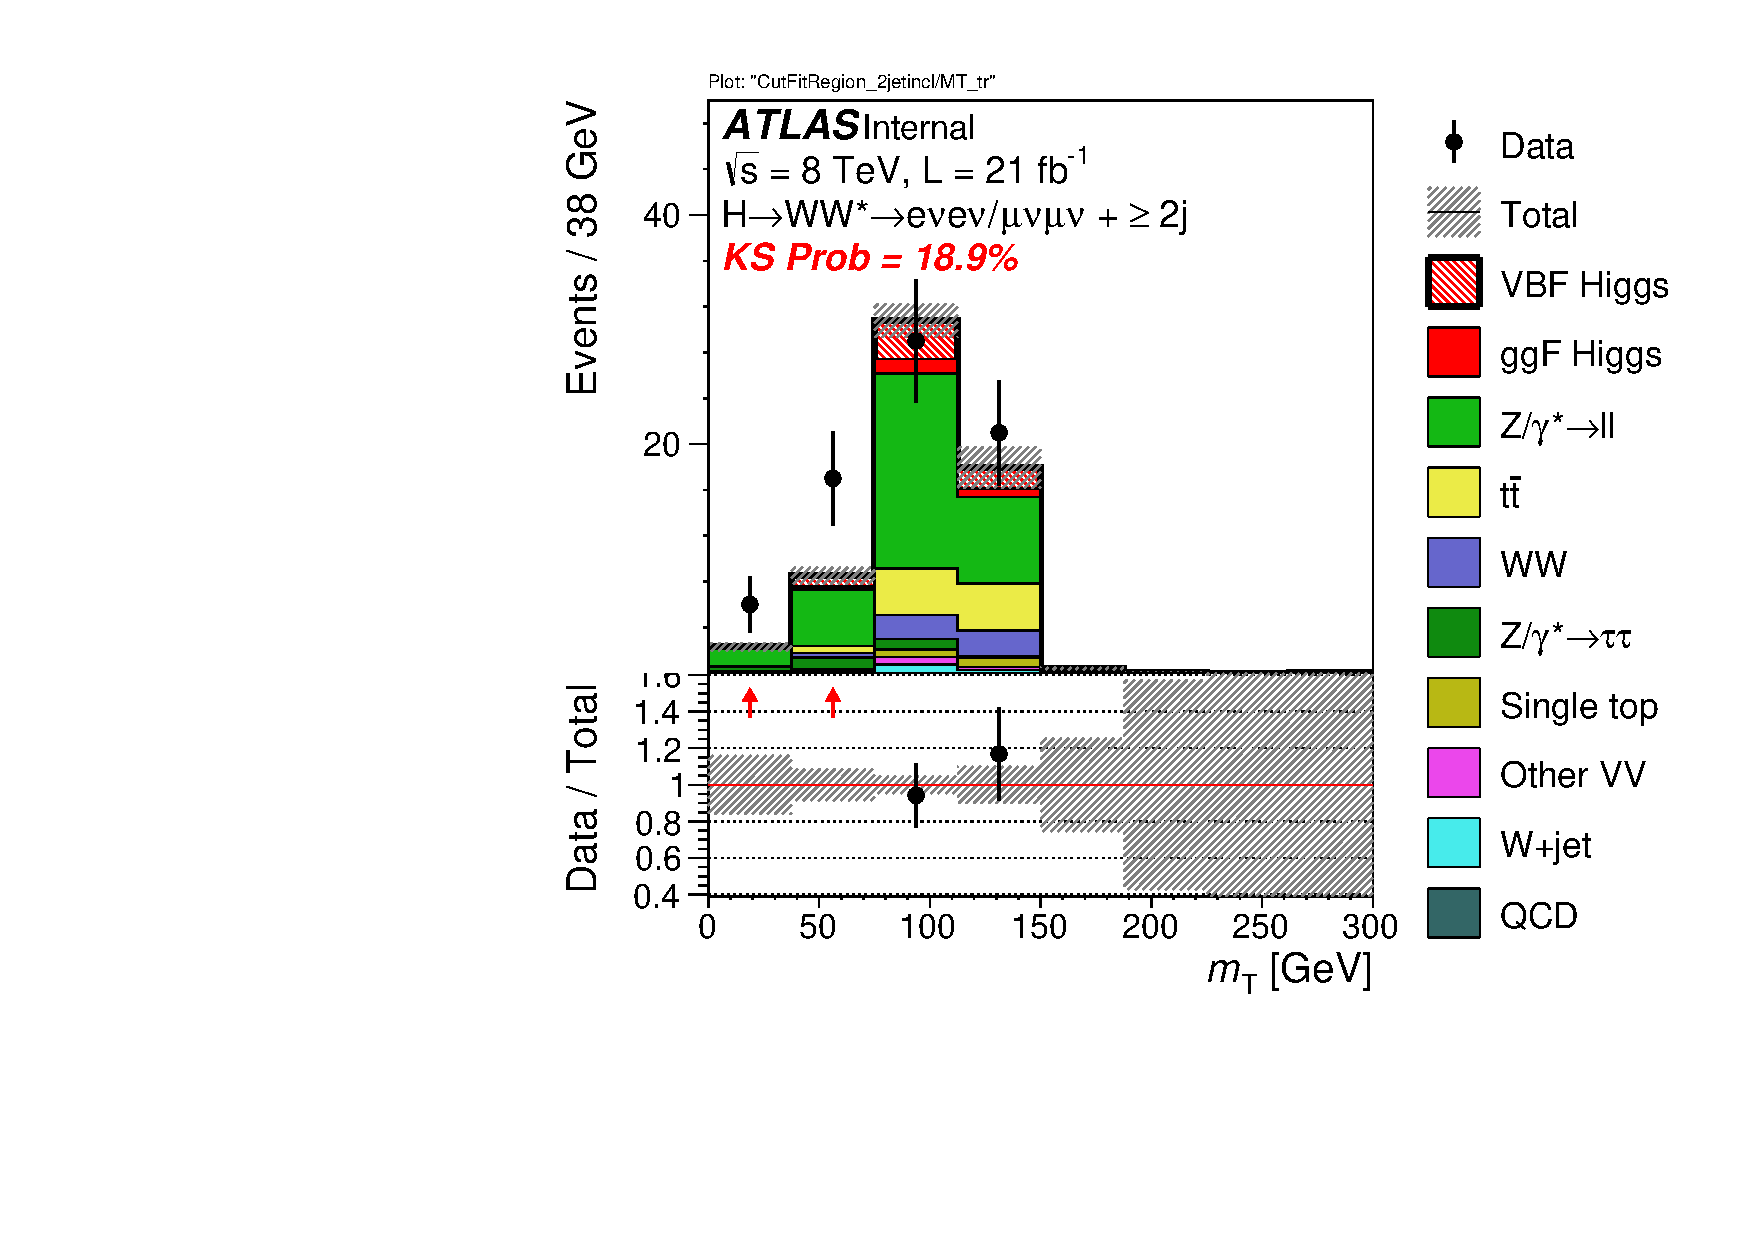
\includegraphics[width=0.4\textwidth]{fig/analysis/BDTinputVarsInSR/SF_SR_FitRegion_MT_tr_mh125_lin.pdf}
   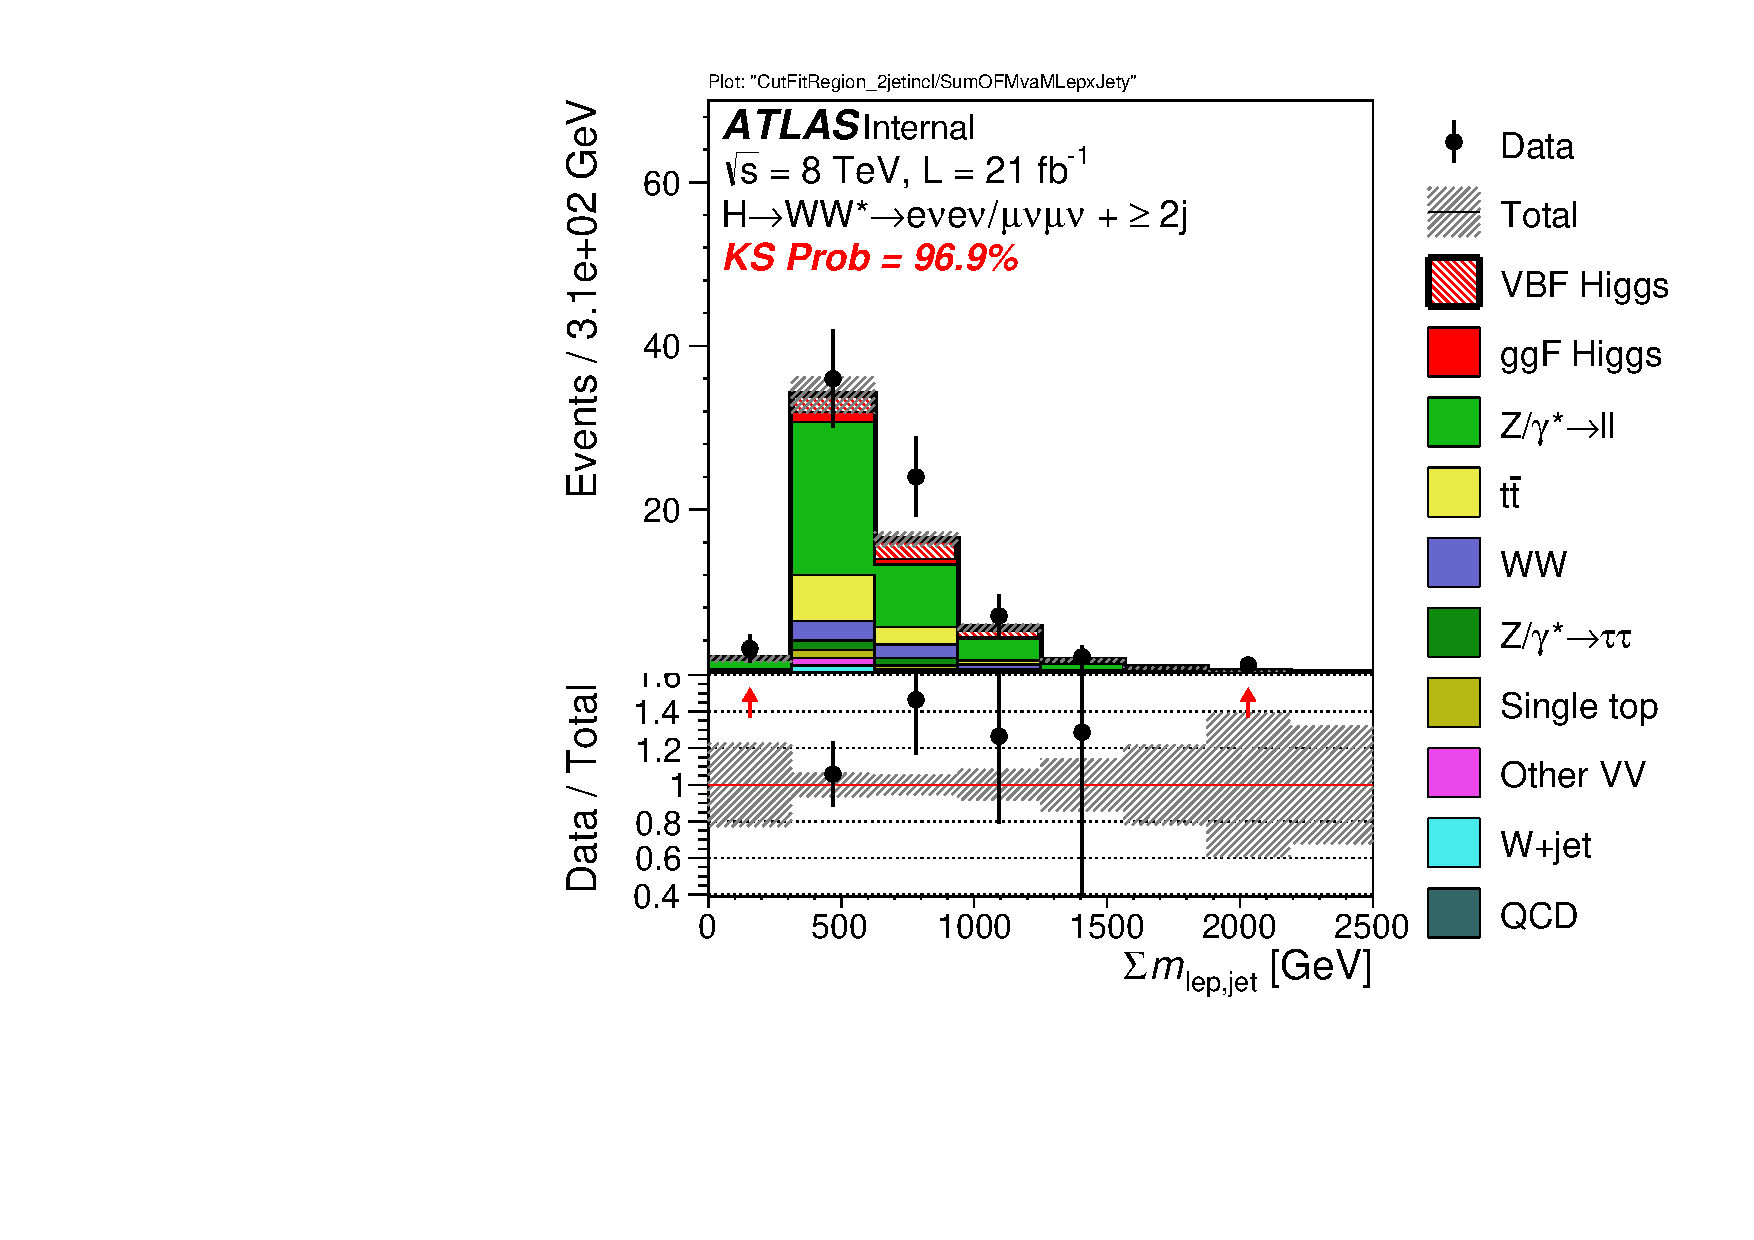
\includegraphics[width=0.4\textwidth]{fig/analysis/BDTinputVarsInSR/SF_SR_FitRegion_SumOFMvaMLepxJety_mh125_lin.pdf}
   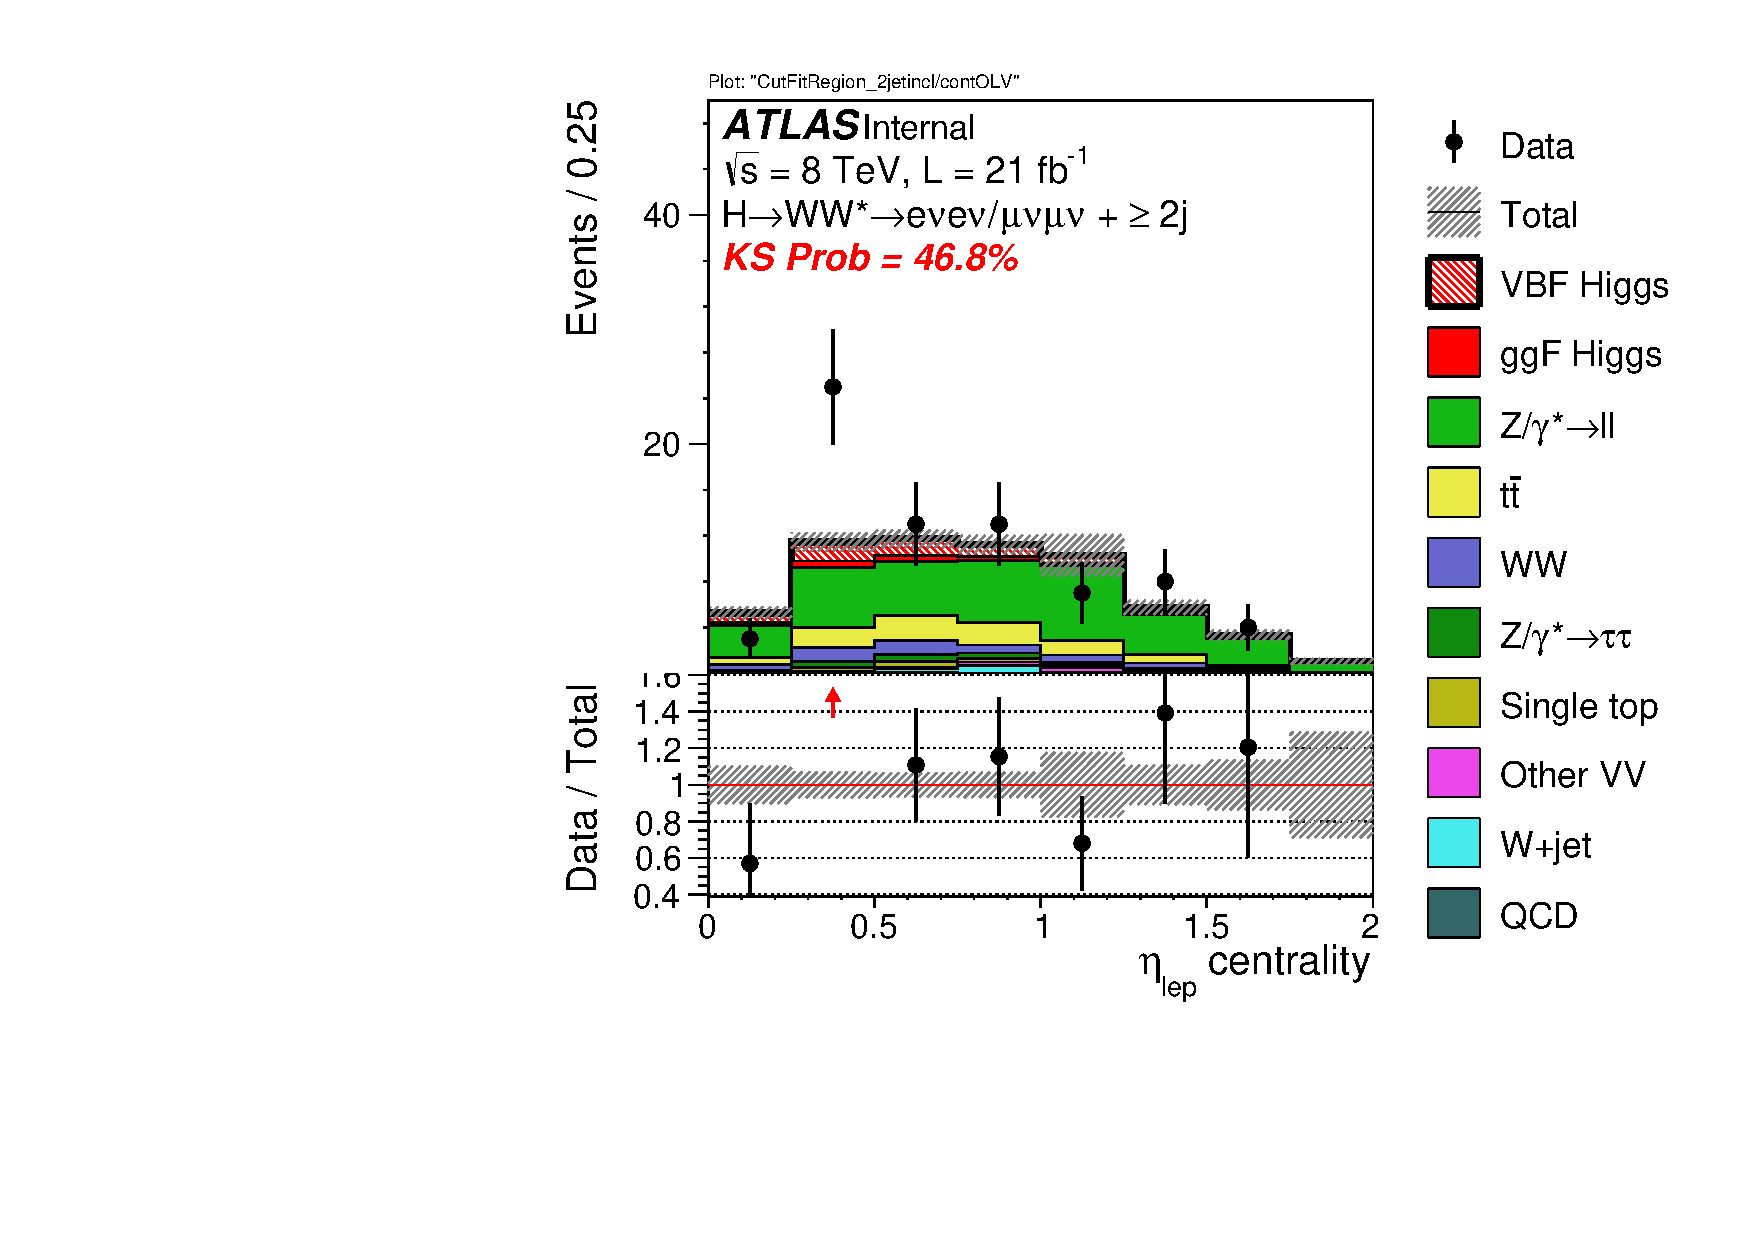
\includegraphics[width=0.4\textwidth]{fig/analysis/BDTinputVarsInSR/SF_SR_FitRegion_contOLV_mh125_lin.pdf}
   \caption{Distributions
   of \dphill, \mll, \dyjj, \mjj, \pTtot, \mT, \SumMlj, and
   \lepEtaCent
   in the \eemm channel in the high BDT fit region ($\textrm{BDT} > -0.48$).}
  \label{chap:analysis:fig:bdt_inputs_sr_sf}
\end{figure}

- cut-based vs. BDT plots shown by Tomo


